\documentclass[12pt,a4paper]{scrartcl} 

%Deutsch:
	\usepackage[ngerman]{babel} %Deutsches Datumformat, Umlaute m\"oglich,...
	\usepackage[utf8]{inputenc}
	\usepackage[T1]{fontenc} 
	
%Quellenverzeichnis:
	\usepackage[maxcitenames=2,autocite=footnote,uniquename=full,uniquelist=true,backend=biber]{biblatex} %style=authoryear-icomp
	\usepackage{csquotes} %Hilfspaket für Biblatex
	\bibliography{bib_database.bib} %Datei mit bibliographischen Daten
	\DefineBibliographyStrings{ngerman}{andothers={et\ al\adddot}} % "u.a." zu "et al."
	\DefineBibliographyStrings{ngerman}{and={\&}} % "und" zu "&"

%Mathematik:
	\usepackage{dsfont} %Symbole
	\usepackage{amsmath} %Umgebung
	\usepackage{amssymb} %Symbole
	\usepackage{bbm} %doppelstreifen bei buchstaben (zb symbol für ganze zahlen \mathbbm{Z})
	
%Grafiken:
	\usepackage{graphics}
	\usepackage{graphicx}
	\usepackage{picinpar} %bilder so einfügen, dass text um bilder weiterläuft
	\usepackage{float} %\begin{figure}[H] => Grafik wird HIER eingefügt!

%Euro-Zeichen:
	\usepackage{eurosym}

%Quellcode:
	%\usepackage[numbered,framed]{mcode} %Quellcode darstellen
	
%Englisch:
	%\usepackage[ngerman,english]{babel} %automatisch erzeugte Überschriften etc. auf englisch
	
\DeclareMathOperator*{\argmin}{arg\,min} % Importiere die Einstellungen aus der Präambel

% hier beginnt der eigentliche Inhalt
\begin{document}

% Deckblatt
\begin{titlepage}
	\rmfamily
	\begin{center}
		% Logo
		%\includegraphics[width=0.15\textwidth]{./logo}\\[1cm]
	
		\textsc{\LARGE Statistisches Consulting}\\[1.5cm]

		\textsc{
			\large{	Master Studiengang Statistik\\[0.25cm]
							Institut für Statistik\\[0.25cm]
							Ludwig-Maximilians-Universität München}}\\[0.25cm]
						
		% Title
		\newcommand{\HRule}{\rule{\linewidth}{0.5mm}}
		\HRule \\[0.4cm]
		{\huge \bfseries Online-Marketing der Interhyp AG\\[0.5cm]Analyse von Tracking-Daten}\\[0.4cm]
		\HRule \\[1.5cm]
		
		% Autoren
		\textbf{Daniel Fuckner} d.fuckner@gmx.de\\
		\textbf{Markus Vogler} markus@vogler-lindau.de\\[1.5cm]
	
		% Betreuer und Projektpartner
		\begin{minipage}{0.4\textwidth}
			\begin{flushleft}
				Projektpartner:\\
				\textbf{Interhyp AG}
			\end{flushleft}
		\end{minipage}
		\hfill
		\begin{minipage}{0.4\textwidth}
			\begin{flushright}
				Betreuer:\\
				\textbf{Dr. Fabian Scheipl}
			\end{flushright}
		\end{minipage}
		
		\vfill

		% Datum
		{\large München, 11.11.2011}
		
	\end{center}
\end{titlepage}

%\thispagestyle{plain}
\pagenumbering{roman} %römische Seitennummerierung

%Abstract
\begin{abstract}
\noindent\subsubsection*{Abstract}
Die Interhyp AG ist Vermittler für private Baufinanzierungen. Das primäre Ziel des Marketing der Interhyp AG ist die Kundenakquise. Da etwa 80\% aller Kundenanträge online abgeschickt werden, liegt der Fokus auf dem Online-Marketing, das über verschiedene Kampagnen verfügt. Beispiele sind Kooperationen mit anderen Unternehmen, bezahlte Anzeigen bei Suchmaschinen oder Bannerschaltungen.\\
Die Refined Labs GmbH ist verantwortlich für das Online-Tracking der Werbekampagnen der Interhyp AG. Durch Online-Tracking werden die Werbekontakte eines potentiellen Kunden zu einem sogenannten Funnel zusammengefasst. Am Ende eines jeden Funnels steht das Ausfüllen eines Onlineantrages oder der Abbruch. Man spricht von konvertierten beziehungsweise nicht-konvertierten Funnels.\\
In dieser Arbeit werden die Tracking-Daten zunächst anhand deskriptiver Analysen vorgestellt. Außerdem werden Methodik und Ergebnisse eines zeitdiskreten Survival-Modells und eines Sequential Pattern Mining-Algorithmus beschrieben. Mit Hilfe des zeitdiskreten Survival-Modells, das mit Stochastic Gradient Boosting geschätzt wurde, konnten Zusammenhänge zwischen den erklärenden Variablen und der Wahrscheinlichkeit für eine Konvertierung gefunden werden. Häufige Abfolgen von Kampagnen in den konvertierten und nicht-konvertierten Funnels wurden mit dem Sequential Pattern Mining-Algorithmus entdeckt. Zudem wurden die Funnels in Form eines Netzwerkes visualisiert. Die Daten für dieses Netzwerk und ein Programm, dass die interaktive Betrachtung ermöglicht, ist im elektronischen Anhang enthalten.
\end{abstract}

%Inhaltsverzeichnis
\newpage
\tableofcontents

\newpage
\pagenumbering{arabic} %ab hier wieder normale Seitennummerierung

% Hier beginnt der eigentliche Text
\section{Einleitung}

Die Interhyp AG ist Vermittler für private Baufinanzierungen. Das heißt, sie wählt aus einem Angebot von verschiedenen Darlehensgebern die optimale Finanzierungsstruktur für einen Kunden aus. Das Unternehmen wurde 1999 von den ehemaligen Goldman-Sachs-Bankern Robert Haselsteiner und Marcus Wolsdorf gegründet. Sechs Jahre später eröffnete die Interhyp AG erste Niederlassungen und konnte gleichzeitig den erfolgreichsten deutschen Börsengang des Jahres verzeichnen. Nach weiteren drei Jahren erfolgte die Übernahme durch ING DIRECT, der weltweilt größten und erfolgreichsten Direktbanken-Gruppe. Heute ist die Interhyp AG der größte Vermittler für private Baufinanzierungen in Deutschland, wurde acht mal in Folge als "Bester Baufinananzierer" (Zeitschrift \euro, Ausgabe 08/2013) ausgezeichnet und verfügt über mehr als 60 Beratungsstandorte mit über 1.000 Mitarbeitern.\\
Das primäre Ziel des Marketing der Interhyp AG ist die Kundenakquise. Da etwa 80\% aller Kundenanträge online abgeschickt werden, liegt der Fokus der Marketing-Abteilung auf dem Online-Marketing, das über verschiedene Kanäle verfügt. Beispiele sind Kooperationen mit anderen Unternehmen wie Immobilienscout24, bezahlte Anzeigen bei Suchmaschinen, Newsletter oder diverse Bannerschaltungen. Durch Online-Tracking können die Werbekontakte eines potentiellen Kunden mit der Interhyp AG zusammengefasst werden. So entsteht ein sogenannter Funnel, wie es in Abbildung \ref{customerJourney} skizziert ist. Jeder potentielle Kunde hat einen oder mehrere aufeinanderfolgende Kontaktpunkte, wobei jeder Kontaktpunkt die genaue Zeit des Kontaktes sowie die Art des Kontaktes, das heißt die Information über welche Kampagne es zu dem Kontakt kam, enthält. Am Ende eines jeden Funnels steht der Abbruch der Beobachtung oder im Idealfall das Ausfüllen eines Onlineantrages durch den Kunden.
\begin{figure}[H]
    \centering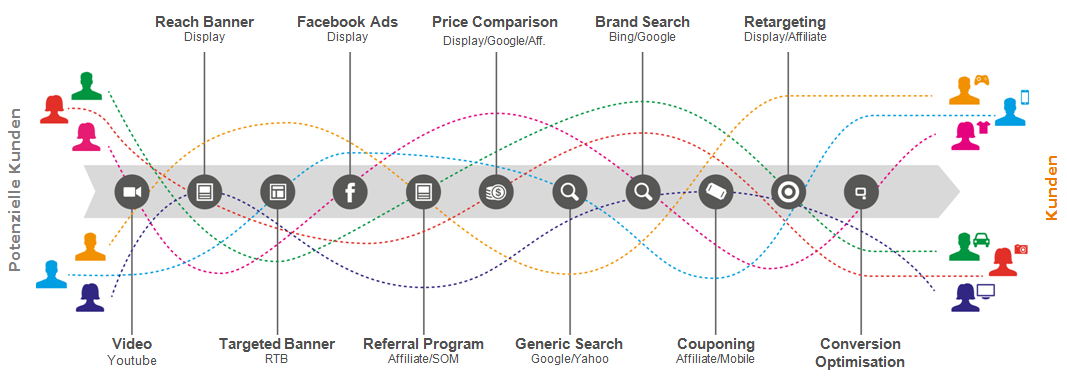
\includegraphics[scale=0.5]{customerJourney.png}\caption[Entstehung eines Funnels]{Entstehung eines Funnels (Quelle: Interhyp AG)}\label{customerJourney}
\end{figure}
\noindent Die Refined Labs GmbH ist auf dem Gebiet des Online-Marketing spezialisiert und verantwortlich für das Online-Tracking der Werbekampagnen der Interhyp AG. Ein Funnel beginnt mit dem ersten Online-Werbekontakt eines potentiellen Kunden mit der Interhyp AG und der damit einhergehenden Erstellung eines Cookies. So können alle weiteren Werbekontakte dem potentiellen Kunden eindeutig zugewiesen werden. Das Tracking endet sobald der potentielle Kunde einen Onlineantrag versendet und damit zum Kunden wird. In diesem Fall spricht man von einem konvertierten Funnel. Wird innerhalb von $90$ Tagen kein Onlineantrag versendet, so wird das Cookie nicht weiter verfolgt und der Funnel wird als nicht-konvertiert bezeichnet.\\
Primäres Ziel dieses Projektes ist das Entdecken von Unterschieden zwischen konvertierten und nicht-konvertierten Funnels. Um dieser Fragestellung gerecht zu werden, wurde ein zeitdiskretes Survival-Modell mittels Stochastic Gradient Boosting geschätzt und ein Sequential Pattern Mining-Algorithmus angewendet. Außerdem wurden die Funnels anhand eines Netzwerkes visualisiert.\\
Die Arbeit ist wie folgt gegliedert. In Kapitel \ref{datenlage} und \ref{descriptiv} werden die Datenaufbereitung und die Variablen erklärt. Daraufhin wird die Methodik des Survival-Modells in Kapitel \ref{survival}, der Sequential Pattern Mining-Algorithmus in Kapitel \ref{spm} und das Netzwerk in Kapitel \ref{network} erläutert. Die Ergebnisse dieser Methoden werden in Kapitel \ref{ergebnisse} vorgestellt und abschließend erfolgt eine Zusammenfassung in Kapitel \ref{zusammenfassung} und die Beschreibung des elektronischen Anhangs in Kapitel \ref{anhang}. % Importiere die Einleitung
\section{Datenlage}\label{datenlage}
%\begin{table}[H]
 %   \begin{center}
  %      \begin{tabular}{|c|p{10cm}|}
   %         \hline $ touchpoint $  & Kontaktpunkt einer Beobachtung \\
    %        \hline $ funnel $ & zeitliche Abfolge der Touchpoints einer Beobachtung\\ 
     %       \hline $ campaign $ & Kategorie der Werbeform auf der obersten Ebene, gegebenfalls auch Ebenen darunter \\ 
      %      \hline $ position \in \{1,2,\dots\}$  & Nummer des Touchpoints eines Funnels\\
       %     \hline $ transaction \in \{0,1\}$  & $1$ steht für konvertiert und $0$ für nicht-konvertiert\\
        %    \hline $ funnelLength \in \{1,2,\dots\} $  & Anzahl der Touchpoints eines Funnels\\
         %   \hline
        %\end{tabular} 
    %\end{center}
    %\caption{Definition der wichtigsten Begriffe}
%\end{table}
Die Daten wurden von der Refined Labs GmbH als SQL-Dump bereitgestellt, der eine Größe von circa $13$ Gigabyte hat. Die MySQL-Datenbank enthält die vier Tabellen \textit{project\_out}, \textit{redirects\_short}, \textit{searchFunnel} und \textit{stage2\_transactionHandling}. Mit Hilfe der vorhanden Informationen in \textit{searchFunnel} und \textit{stage2\_transactionHandling} konnten die Kontaktpunkte in \textit{redirects\_short} in konvertierte und nicht-konvertierte Funnels unterteilt werden. In \textit{projects\_out} sind die Kampagnen in Form einer Baumstruktur organisiert. In Absprache mit der Interhyp AG wurden $17$ Kategorien ausgewählt, die sich auf den ersten drei Ebenen dieser Baumstruktur befinden. Anhand von IDs wurde jedem Kontaktpunkt eine dieser Kategorien zugewiesen.\\
Tabelle \ref{exdata} enthält ein Datenbeispiel mit den Spalten \textit{ID}, \textit{Campaign}, \textit{Transaction}, \textit{First} und \textit{Last}. Das Beispiel enthält zwei verschiedene \textit{IDs}, das heißt zwei Funnels, wobei der erste vier und der zweite drei Kontaktpunkte hat. Die Spalte \textit{Campaign} enthält die Kampagne der Kontaktpunkte. \textit{Transaction}, \textit{First} und \textit{Last} sind binäre Variablen. \textit{Transaction} gibt an, ob der Kunde konvertiert ist, wobei der Wert $1$ nur für den letzten Kontaktpunkt vor der Konvertiertung angenommen wird. Das heißt bei \textit{ID} $1$ handelt es sich um einen konvertierten und bei \textit{ID} $2$ um einen nicht-konvertierten Funnel. \textit{First} beziehungsweise \textit{Last} nimmt den Wert $1$ an, wenn es sich um den ersten beziehungsweise letzten Kontaktpunkt eines Funnels handelt. Die $17$ Kampagnen und weitere Features, die aus den Daten erzeugt wurden, werden in Kapitel \ref{descriptiv} näher erläutert.\\
\begin{table}[H]
	\begin{center}
		\begin{tabular}{|c|l|c|c|c|c|}
			\hline
			ID & Campaign 									 & Transaction & First & Last & ... \\ \hline\hline
			1  & Affiliate - Partnerprogramm & 0					 & 1		 & 0    & ... \\ \hline
			1  & SEM - Brand                 & 0					 & 0		 & 0    & ... \\ \hline
			1  & Direct                      & 0					 & 0		 & 0    & ... \\ \hline
			1  & Direct                      & 1					 & 0		 & 1    & ... \\ \hline
			2  & Display                     & 0					 & 1		 & 0    & ... \\ \hline
			2  & SEM - Generisch             & 0					 & 0		 & 0    & ... \\ \hline
			2  & Social Media                & 0					 & 0		 & 1    & ... \\ \hline
		\end{tabular} 
	\end{center}
	\caption{Beispiel für einen Auszug aus der Datenbank}\label{exdata}
\end{table}
Ein Kontaktpunkt ist entweder ein \textit{Click} oder ein \textit{View}. Man spricht von einem \textit{Click}, wenn der potentielle Kunde tatsächlich etwas angeklickt hat, wobei die genaue Definition von der Kampagne abhängt. Ein \textit{View} wird getrackt, wenn ein Banner oder ähnliches lediglich gesehen, aber nicht angeklickt wird. An dieser Stelle wirft die Datenerhebung allerdings ein Problem für die statistischen Analysen auf. Die \textit{Views} werden für alle konvertierten Funnels gespeichert, für die nicht-konvertierten Funnels allerdings nur, wenn diese bei einem anderen Kunden der Refined Labs GmbH konvertieren. Dass heißt, es ist eine systematische Veränderung der Daten gegeben. Deshalb besteht keine Möglichkeit die \textit{Views} in statistische Analysen, die konvertierte und nicht-konvertierte Funnels vergleichen, einzubeziehen. Die \textit{Views} werden lediglich in Kapitel \ref{descriptiv} in einigen Plots betrachtet, die nur konvertierte Funnels enthalten, und von den weiteren Analysen ausgeschlossen.\\
Nach der Vorverarbeitung der Daten liegen ??? konvertierte und ??? nicht-konvertierte Funnels vor, die nur \textit{Clicks} enthalten. Eine nähere Beschreibung der erstellten Features erfolgt in Kapitel \ref{descriptiv}.




\section{Deskriptive  Analyse}\label{descriptiv}

Tabelle \ref{varbeschreibung} enthält eine Übersicht mit den erzeugten Variablen. Diese werden in diesem Kapitel näher betrachtet. Als Position wird im folgenden die Nummer eines Kontaktpunktes innerhalb eines Funnels bezeichnet. Das heißt für jeden Funnel nimmt der erste Kontakt die Position $1$ an. Die Abbildungen wurden mit dem \textit{R}-Paket \textit{ggplot2} \cite{ggplot2} erzeugt.
\begin{table}[H]
    \begin{center}
\begin{tabular}{|c|p{10cm}|}
		\hline $ clickCount \in \mathbb{N} $ & Anzahl an \textit{Clicks} bis zur aktuellen Position\\
    \hline $ hasClicked\in\{0,1\} $  & Dummyvariable, die angibt ob vor der aktuellen Position schon geklicked wurde ($1$) oder nicht ($0$). \\
		\hline $ campaign $ & Kampagne der aktuellen Position\\ 
    \hline $ campaignLast $ & Kampagne der vorherigen Position\\ 
    \hline $ campaignLast2 $  & Kampagne der vorletzten Position\\
    \hline $ weekday \in \{Montag,...\}$ & Wochentag des Kontaktes  \\
    \hline $ hour \in \{0,1,\dots, 23\} $  & Uhrzeit des Kontaktes \\
    \hline $ timeSinceLast \in \mathbb{R}$  & Zeitdifferenz zwischen aktueller und vorheriger Position\\
    \hline $ timeSinceFirst \in \mathbb{R} $ & Zeitdifferenz zwischen aktueller und erster Position\\
    \hline$ freq \in \mathbb{R} $ & Frequenz der Kontaktpunkte in einem Funnel\\
    \hline
\end{tabular} 
 \end{center}
 \caption{Variablenbeschreibung}\label{varbeschreibung}
\end{table}

\subsection{Views in den konvertierten Funnels}\label{plotsViews}

\subsubsection*{clickCount}
Aufgrund der in Kapitel \ref{datenlage} beschriebenen Problematik bei der Datenerhebung der \textit{Views} können die Variablen \textit{clickCount} und \textit{hasClicked} nur in den konvertierten Funnels betrachtet werden.
\begin{figure}[H]
    \centering
    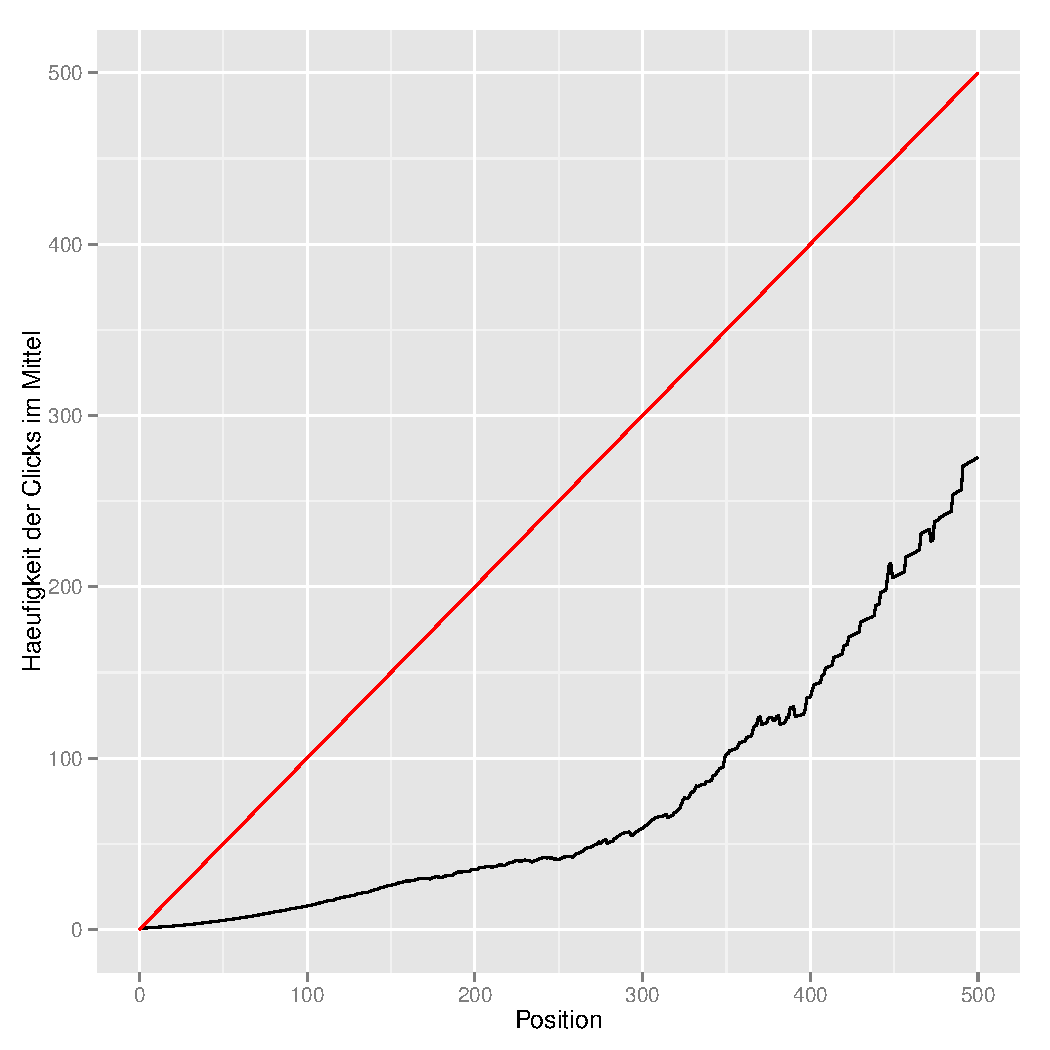
\includegraphics[scale=0.5]{clickCountSucc.pdf}
    \caption[Häufigkeit der Clicks im Mittel]{Häufigkeit der Clicks im Mittel für jede Position}
    \label{clickCount}
\end{figure}
\noindent In Abbildung \ref{clickCount} ist der \textit{clickCount} dargestellt. Auf der $x$-Achse ist die Position aufgetragen und auf der $y$-Achse der \textit{clickCount}, das heißt die Häufigkeit der \textit{Clicks} gemittelt über alle konvertierten Funnels für jede Position. Die rote Diagonale wäre erreicht, wenn die konvertierten Funnels nur aus \textit{Clicks} bestehen würden. Es ist zu erkennen, dass die Linie mit der Position ansteigt. An Position $100$ ist die mittlere Anzahl der Clicks 13.7, das heißt im Mittel bestehen die ersten $100$ Kontakte eines Funnels aus $14$ \textit{Clicks} und $86$ \textit{Views}. Die Anzahl der \textit{Views} übersteigt die Anzahl der \textit{Clicks} also deutlich.\\

\subsubsection*{hasClicked}
Die Variable \textit{hasClicked} (siehe Abbildung \ref{hasClicked}) gibt für jede Position den Anteil der Funnels an, die bis dorthin mindestens einen \textit{Click} enthalten. Dieser Wert nimmt zwischen Position $1$ und Position $7$ ab. Dies ist dadurch zu erklären, dass es viele Funnels gibt, die \textit{Clicks} enthalten und deren Länge kleiner als $6$ ist. Sobald diese Funnels beendet sind, werden sie an der nächsten Position selbstverständlich nicht mehr berücksichtigt. Ab Position $7$ steigt die Kurve dann bis zur $1$ an. Ein Wert von $1$ bedeutet, dass alle Funnels bereits einen \textit{Click} hatten.
\begin{figure}[H]
    \centering
    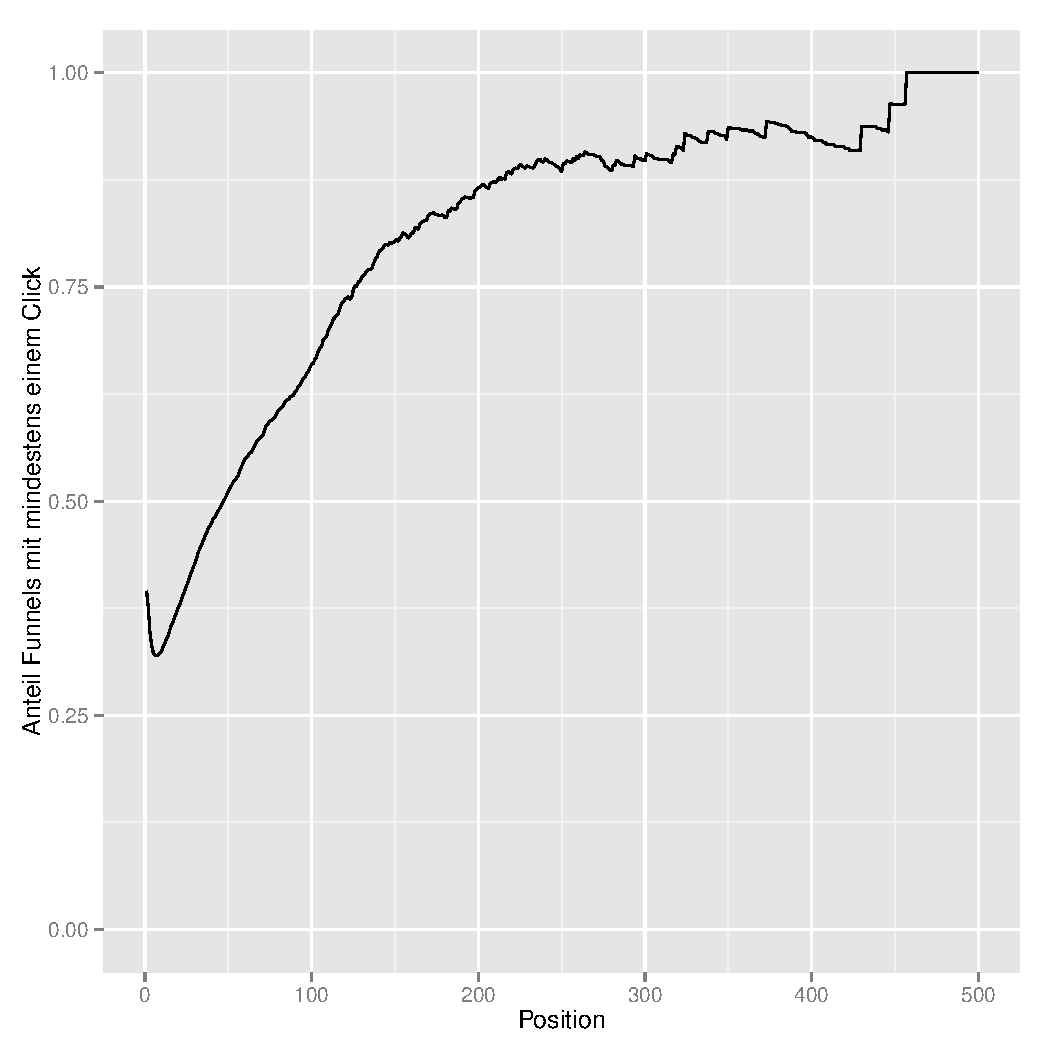
\includegraphics[scale=0.5]{hasClickedSucc.pdf}
    \caption[Anteil Funnels mit mindestens einem Click]{Anteil der Funnels mit mindestems einem Click für jede Position}
    \label{hasClicked}
\end{figure}

\subsubsection*{campaign}
In Kapitel \ref{datenlage} wurde bereits eine Übersicht über die Kampagnen gegeben. Abbildung \ref{campaignSucc} enthält die Verteilung dieser $17$ Kategorien in den konvertierten Funnels, das heißt auf der $x$-Achse ist die relative Häufigkeit aufgetragen und auf der $y$-Achse die Kategorien. Die orangefarbigen Balken repräsentieren die Verteilung in den konvertierten Funnels nur mit \textit{Clicks}, wie sie auch in den späteren Analysen verwendet werden. Die blauen Balken enthalten \textit{Clicks} und \textit{Views}.\\
Es ist zu erkennen, dass die Kampagne \textit{Display} bei den Funnels mit \textit{Views} $84 \%$ der gesamten Kontaktpunkte ausmacht. Das heißt die Bannerschaltungen überwiegen deutlich und ansonsten hat nur \textit{Direct} einen Anteil von über $5 \%$.\\
Werden die \textit{Views} nicht berücksichtigt so verteilen sich die Kampagnen besser. \textit{Display} macht jetzt weniger als $10 \%$ aus und \textit{Direct} ist mit über $35 \%$ die am häufigsten auftretende Kampagne. Außerdem haben auch \textit{SEO}, \textit{SEM - Generisch}, \textit{SEM - Brand}, \textit{Kooperationen - Immoscout24} und \textit{Affiliate - Partnerprogramm} einen Anteil von über $5 \%$. Die restlichen Kampagnen, besonders \textit{Social Media}, machen nur einen kleinen Teil der Daten aus.
\begin{figure}[H]
    \centering
    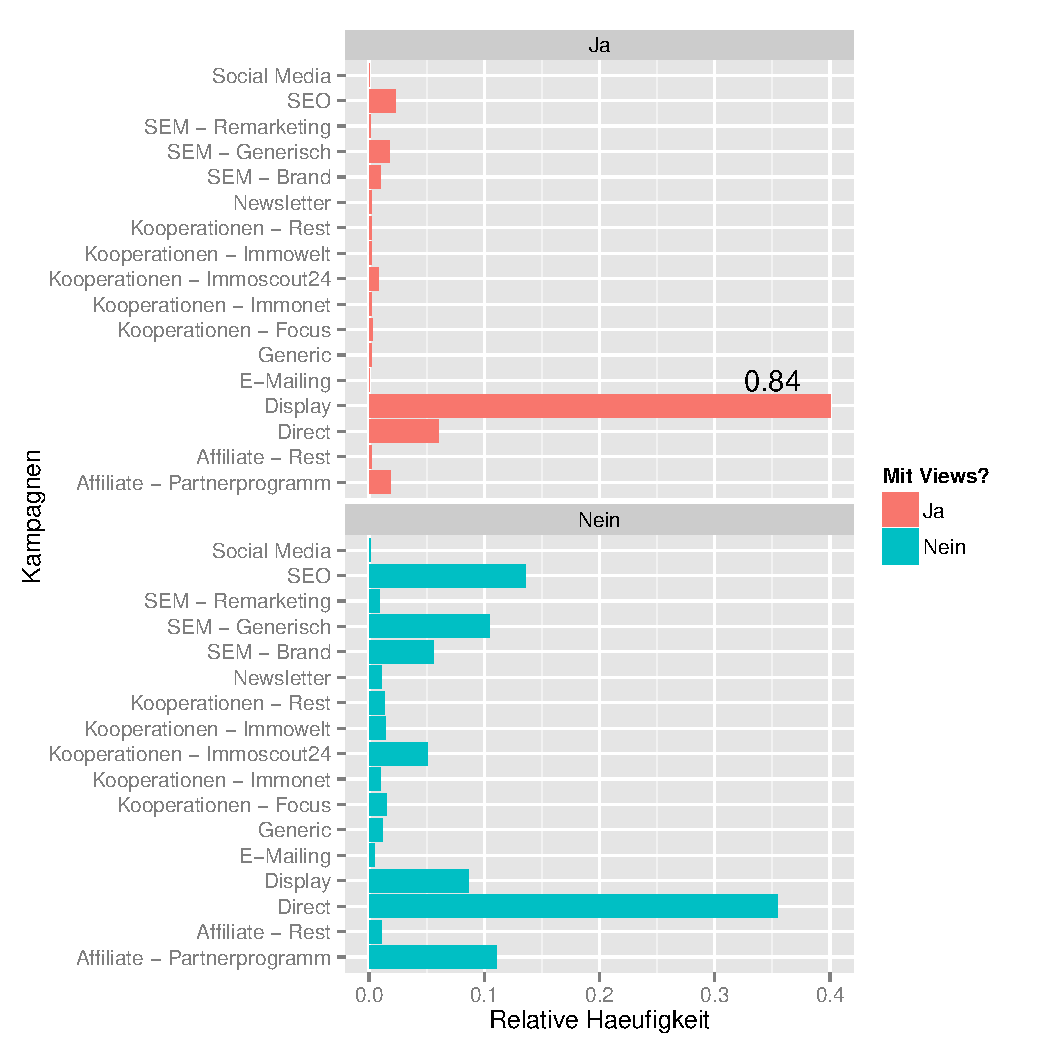
\includegraphics[scale=0.6]{campaignSucc.pdf}
    \caption[Kampagnen der konvertierten Funnels]{Kampagnen der konvertierten Funnels mit und ohne Views}
    \label{campaignSucc}
\end{figure}

\subsection{Vergleich von konvertierten und nicht-konvertierten Funnels}

Nachdem bis hierhin nur die konvertierten Funnels mit Augenmerk auf den \textit{Views} betrachtet wurden, sollen in diesem Kapitel die konvertierten und nicht-konvertierten Funnels miteinander verglichen werden. Das heißt, die \textit{Views} werden von nun an nicht mehr in die Analysen mit einbezogen.

\subsubsection*{weekday}
Die Variable \textit{Weekday} gibt an, an welchem Wochentag ein Konaktpunkt aufgetreten ist. Abbildung \ref{weekday} enthält diesbezüglich Histogramme. Die orangefarbigen Balken entsprechen den konvertierten und die blauen Balken den nicht-konvertierten Funnels. Für weitere Plots in diesem Kapitel gelten die selben Farben. Außerdem ergeben die blauen und orangefarbigen Balken erneut aufsummiert jeweils eins, das heißt sie spiegeln die Verteilung wieder.\\
Es ist zu erkennen, dass die Häufigkeit der Kontaktpunkte von Montag bis Samstag sinkt. Dieser Trend ist in den konvertierten Funnels etwas stärker. Dort sinkt die relative Häufigkeit von $ 0.17 $ am Montag auf $ 0.09 $ am Samstag. Bei den nicht-konvertierten Funnels sinkt die relative Häufigkeit von $ 0.15 $ am Montag auf $ 0.11 $ am Samstag. Außerdem ist der Sonntag bei den nicht-konvertierten mit Abstand der stärkste Tag, während in den konvertierten Funnels der Montag etwas stärker ist als der Sonntag.
\begin{figure}[H]
    \centering
    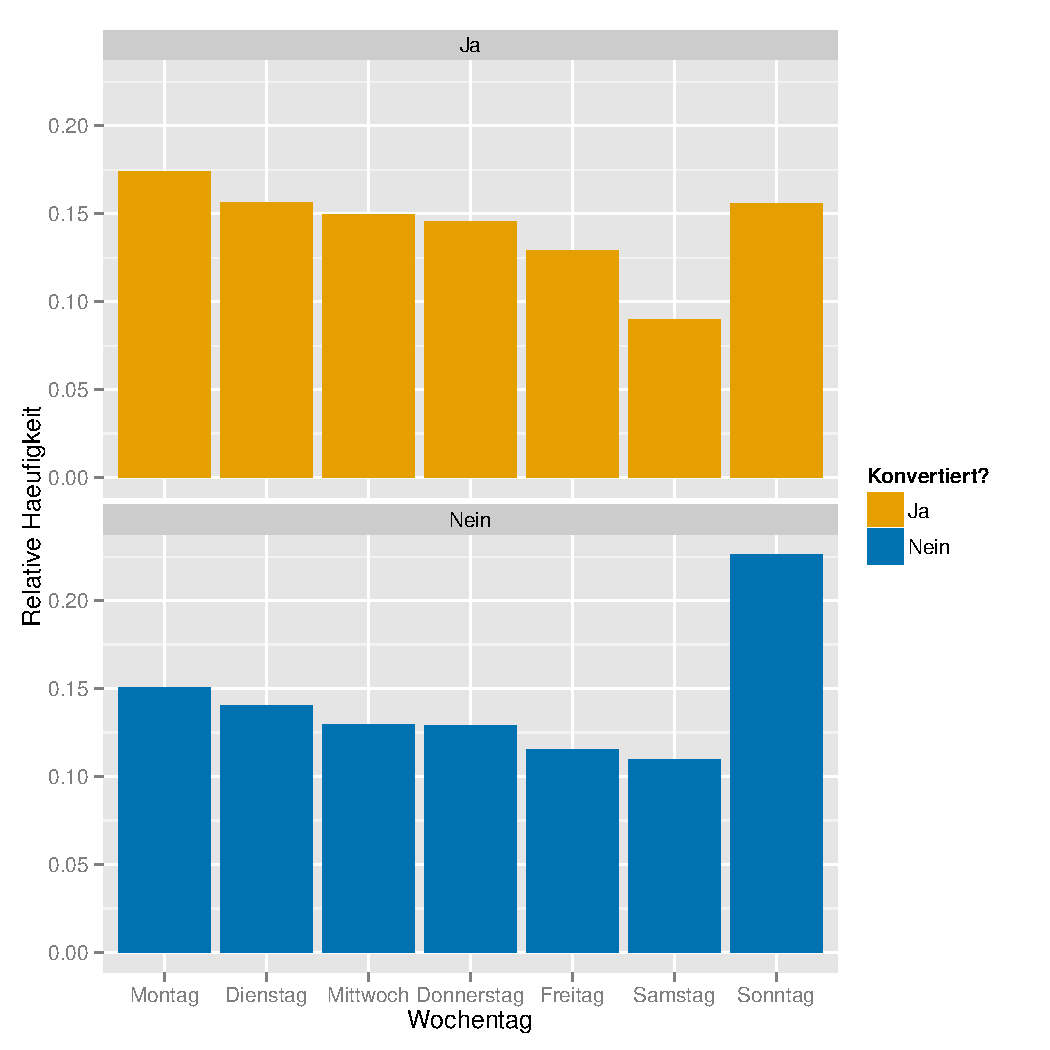
\includegraphics[scale=0.6]{weekday.pdf}
    \caption{Wochentage der Kontaktpunkte}
    \label{weekday}
\end{figure}

\subsubsection*{hour}
Analog zu der Abbildung mit den Wochentagen, enthält Abbildung \ref{hour} Informationen zu der Uhrzeit der Kontaktpunkte in konvertierten und nicht-konvertierten Funnels. Hierfür wurden die Minutenangaben der Uhrzeit jeweils abgeschnitten, so dass \textit{hour} nur die Werte $0,1,...,23$ annehmen kann.\\
\begin{figure}[H]
    \centering
    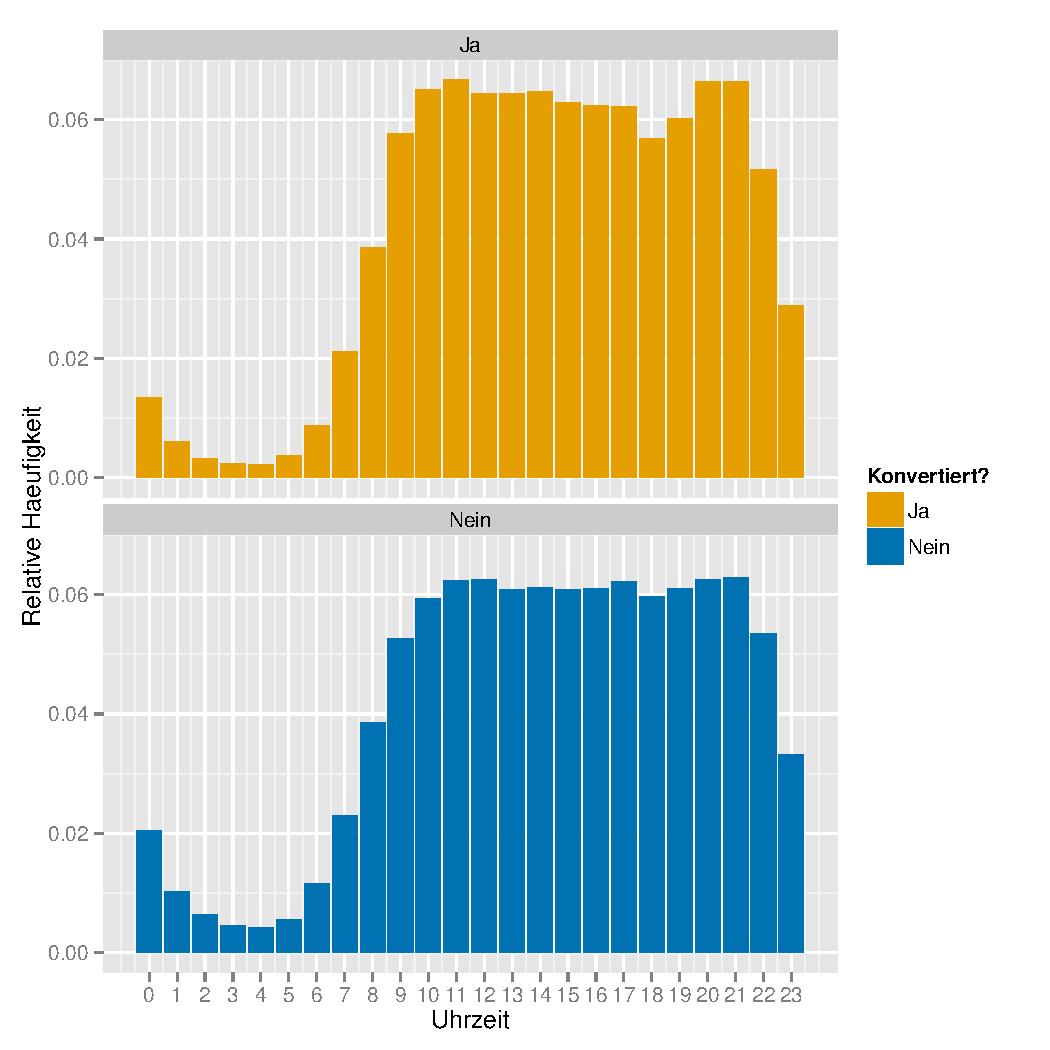
\includegraphics[scale=0.6]{hour.pdf}
    \caption{Uhrzeit der Kontaktpunkte}
    \label{hour}
\end{figure}
\noindent Die Verteilungen in konvertierten und nicht-konvertierten Funnels sind sich sehr ähnlich, so dass keine deutlichen Unterschiede erkennbar sind. Insgesamt kann man zusammenfassen, dass in der Nacht zwischen zwei und sechs Uhr sehr wenige Kontaktpunkte stattfinden. Ab sechs Uhr steigt die relative Häufigkeit der Kontaktpunkte bis circa elf Uhr an und dann bleibt sie konstant bis circa $21$ Uhr. Daraufhin fällt die relative Häufigkeit wieder ab. Dies ist lediglich darauf zurück zu führen, dass nachts weniger Menschen online sind.

\subsubsection*{campaign}
Wie bereits in Kapitel \ref{plotsViews} werden die verschiedenen Kampagnen betrachtet. Allerdings werden an dieser Stelle die konvertierten und nicht-konvertierten Funnels miteinander verglichen, wobei die \textit{Views} nicht berücksichtigt werden (siehe Abbildung \ref{campaign}). Das heißt, die Verteilung der konvertierten Funnels ohne \textit{Views} aus Kapitel \ref{plotsViews} entspricht der Verteilung der konvertierten Funnels in diesem Abschnitt. Eine nähere Beschreibung der unterschiedlichen Kampagnen ist in Abbildung \ref{beschreibungCampaign} zu finden.\\
Die Verteilung in den konvertierten Funnels wurde bereits in Kapitel \ref{plotsViews} etwas näher beleuchtet. Während dort \textit{Direct} mit Abstand die stärkste Kampagne ist, sind in den nicht-konvertierten Funnels \textit{Affiliate - Partnerprogramm} und \textit{Display} die stärksten Kategorien und \textit{Direct} ist lediglich drittstärkste mit einer relativen Häufigkeit von $ 0.123 $. Wie in den konvertierten Funnels haben hier auch \textit{SEO}, \textit{SEM - Generisch} und \textit{Kooperationen - Immoscout24} einen Anteil von über $5 \%$. \textit{SEM - Brand} tritt in den konvertierten Funnels deutlich häufiger auf als in den nicht-konvertierten. Für die restlichen Kampagnen liegen insgesamt wenige Daten vor.

\begin{figure}[H]
	\centering
	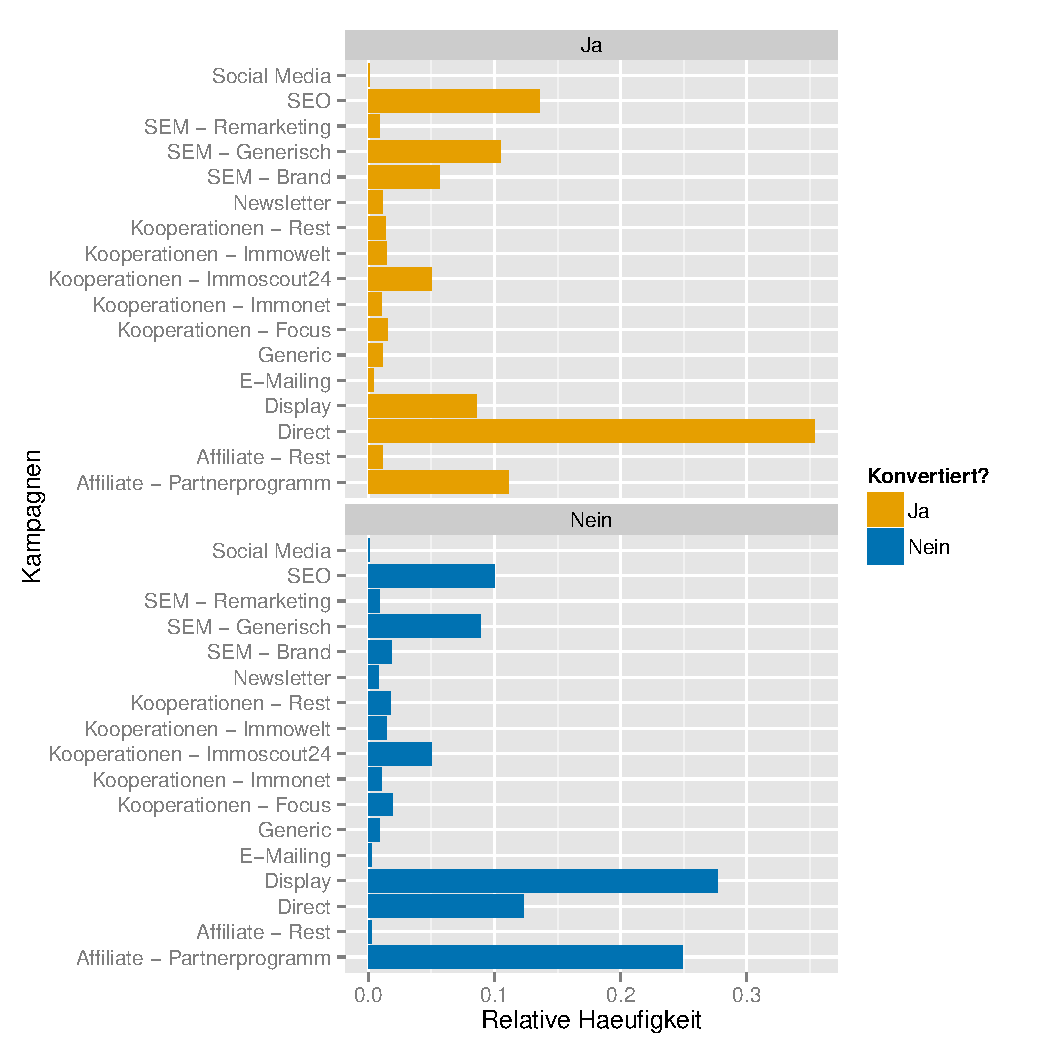
\includegraphics[scale=0.6]{campaign.pdf}
	\caption{Kampagnen der konvertierten und nicht-konvertierten Funnels}
	\label{campaign}
\end{figure}
    
\subsubsection*{funnelLength}
Die \textit{funnelLength} gibt die Anzahl der Kontaktpunkte eines Funnels an. In Abbildung \ref{funnelLength} sind nur diejenigen Funnels dargestellt, deren Länge $20$ Kontaktpunkte nicht überschreitet, da es, relativ gesehen, sehr wenige längere Funnels gibt.\\
Von den nicht-konvertierten Funnels haben $75 \%$ nur einen Kontaktpunkt. Von dort nimmt die relative Häufigkeit der Funnels mit steigender Länge sehr schnell ab. Von den konvertierten Funnels haben $41 \%$ nur einen Kontaktpunkt. Das heißt, relativ betrachtet, gibt es dort mehr Funnels mit mehreren Kontaktpunkten. Allerdings gibt es insgesamt deutlich mehr nicht-konvertierte als konvertierte Funnels, so dass die absoluten Anzahl für die nicht-konvertierten stets größer ist. Der Mittelwert beziehungsweise der Median der Länge der Funnels ist bei den konvertierten Funnels $4.1$ beziehungsweise $2$ und bei den nicht-konvertierten $1.66$ beziehungsweise $1$. 

\begin{figure}[H]
    \centering
    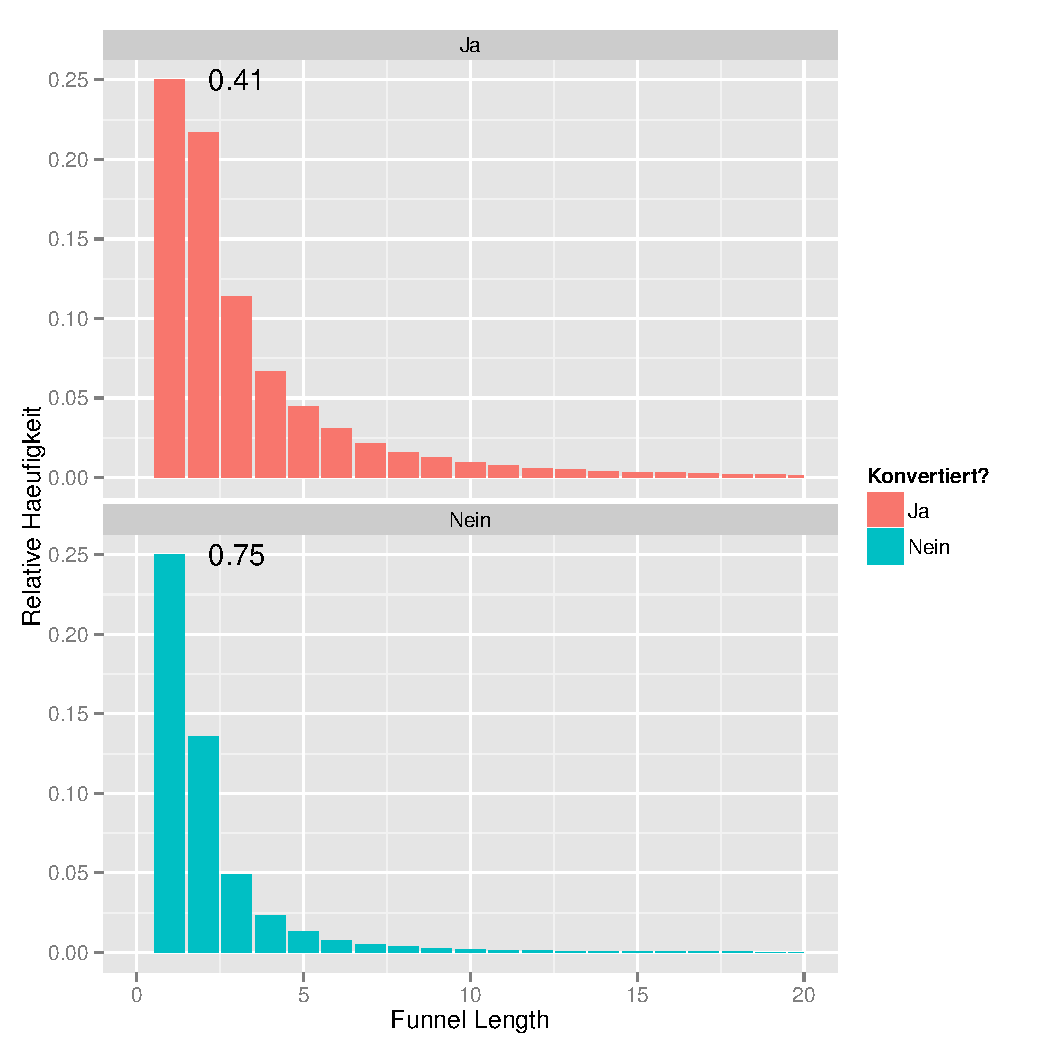
\includegraphics[scale=0.6]{funnelLength_First.pdf}
    \caption[Länge der Funnels]{Länge der Funnels in konvertierten und nicht-konvertierten Funnels}
    \label{funnelLength}
\end{figure}

\subsubsection*{timeSinceFirst}
Das Feature \textit{timeSinceFirst} gibt für jede Position die verstrichene Zeit seit dem ersten Kontaktpunkt an. In Abbildung \ref{timeSinceFirst} wird dieses nur für die letzte Position der Funnels geplottet, so dass die Gesamt-Beobachtungsdauer der Funnels betrachtet wird, das heißt die verstrichene Zeit zwischen dem ersten und dem letzten Kontaktpunkt eines jeden Funnels. Auf der $x$-Achse ist die Beobachtungsdauer in Tagen von $0$ bis $50$ aufgetragen.\\
Hier gestaltet sich ein ähnliches Bild wie in Abbildung \ref{funnelLength}. Allerdings muss berücksichtigt werden, dass die \textit{timeSinceFirst} für die erste Position nicht existiert und somit hier nicht berücksichtigt wird. Von den nicht-konvertierten Funnels haben $58 \%$ eine Beobachtungsdauer von weniger als einem Tag. Längere Beobachtungsdauern treten deutlich seltener auf. Von den konvertierten Funnels haben $33 \%$ eine Beobachtungsdauer von weniger als einem Tag und längere Beobachtungsdauern treten, relativ betrachtet, häufiger auf als in den nicht-konvertierten Funnels.\\
Auffällig sind außerdem die Hückel, die im Rhythmus von sieben Tagen auftreten. Dies ist darauf zurückzuführen, dass Sonntag und Montag die zwei Tage mit den häufigsten Kontakten sind und beispielsweise Bannerschaltungen am Wochenende besonders häufig eingesetzt werden. Bei den konvertierten Funnels liegt der Mittelwert der Beobachtungsdauer bei $21.1$ Tagen und bei den nicht-konvertierten Funnels bei $5.3$ Tagen. 
\begin{figure}[H]
    \centering
    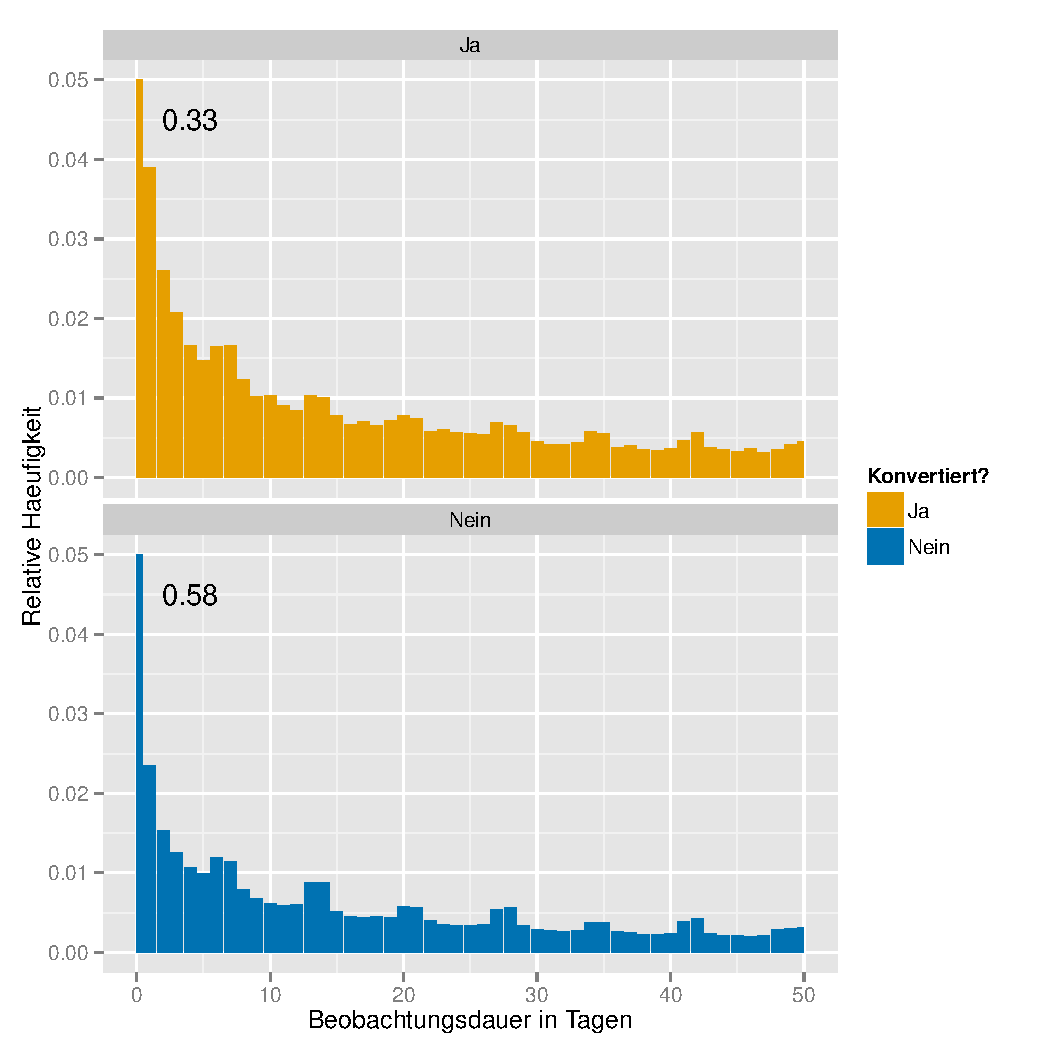
\includegraphics[scale=0.6]{timeSinceFirst_Last.pdf}
    \caption[Beobachtungsdauer in Tagen]{Beobachtungsdauer in Tagen der konvertierten und nicht-konvertierten Funnels}
    \label{timeSinceFirst}
\end{figure}

\subsubsection*{timeSinceLast}
Die Variable \textit{timeSinceLast} gibt die verstrichene Zeit zwischen zwei aufeinander folgenden Kontaktpunkte an. Diese ist in Abbildung \ref{timeSinceLast} abgebildet, wobei nun alle Kontaktpunkte berücksichtigt werden und nicht nur der letzte, wie es bei \textit{timeSinceFirst} der Fall war.\\
Die relative Häufigkeit der Abstände, die kürzer als ein Tag sind ist bei den nicht-konvertierten Funnels höher als bei den konvertierten. Ansonsten sind die Werte bei den konvertierten Funnels höher, wobei wieder ein Abfall mit der Zeit und eine wöchentlich Periodizität zu erkennen sind.\\
Da hier nur die Verteilungen jeweils innerhalb der konvertierten und nicht-konvertierten Funnels verglichen werden, ist \textit{timeSinceLast} keine geeignetes Maß zum Vergleich der Frequenzen der Kontaktpunkte. Dafür wurde die Variable \textit{freq} erzeugt, die im nächsten Abschnitt beschrieben wird.
\begin{figure}[H]
    \centering
    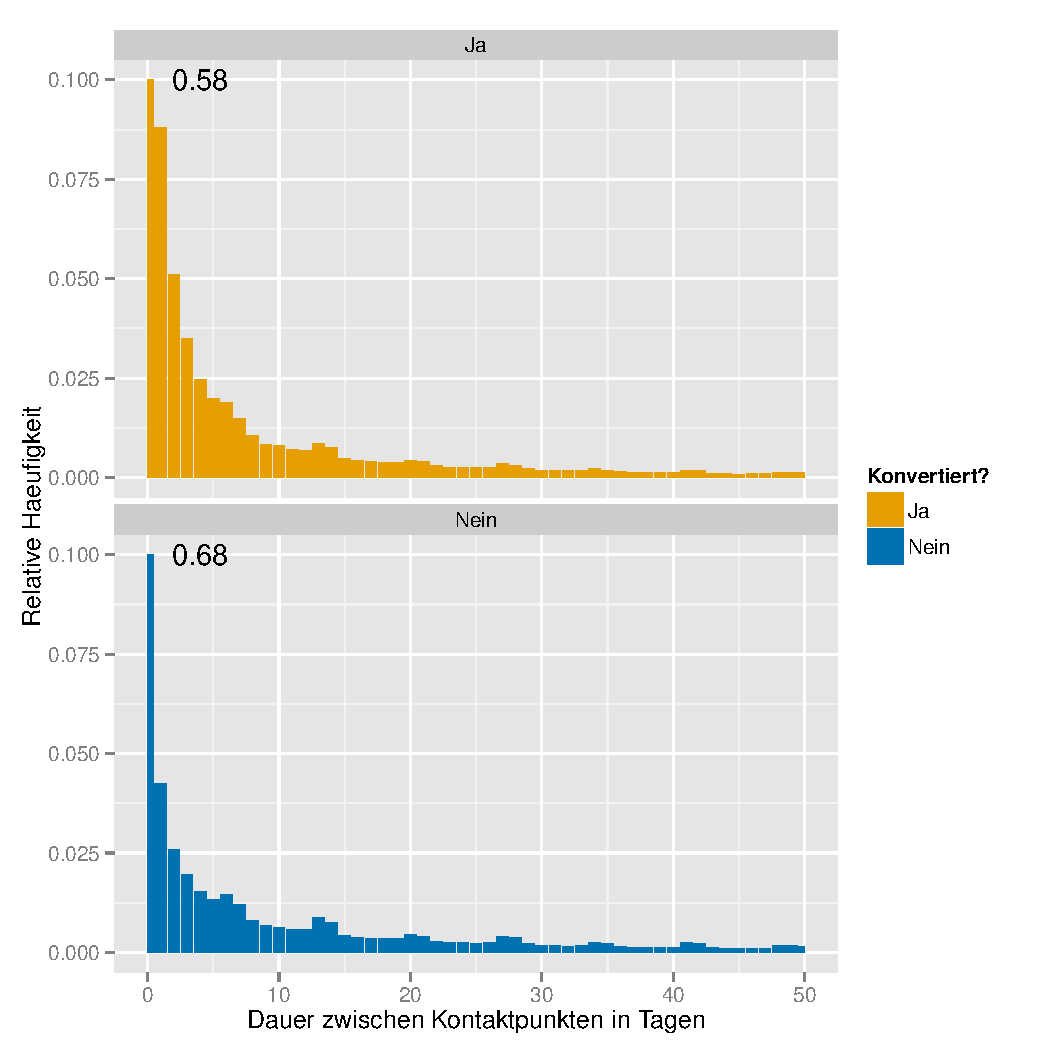
\includegraphics[scale=0.6]{timeSinceLast.pdf}
    \caption[Dauer zwischen zwei Kontaktpunkten]{Dauer zwischen zwei Kontaktpunkten in den konvertierten und nicht-konvertierten Funnels}
    \label{timeSinceLast}
\end{figure}

\subsubsection*{freq}
Die Frequenz wird wie folgt berechnet. Die Daten werden dahingehend gefiltert, dass für jeden Funnel nur der letzte Kontaktpunkt vorhanden ist. Die Variable \textit{timeSinceFirst} gibt somit wieder die Beobachtungsdauer des gesamten Funnels an. Daraufhin wird die Länge des Funnels (siehe Abbildung \ref{funnelLength}) durch die Beobachtungsdauer in Stunden geteilt, so dass eine Größe ensteht, die angibt, wieviel Kontaktpunkte der jeweilige Funnel pro Stunde hatte. Diese Frequenz wird in Abbildung \ref{freq} abgebildet, wobei auf der $x$-Achse die Länge der Funnels zwischen vier und $25$ aufgetragen ist. Für Funnels mit einem Kontaktpunkt existiert offentsichtlich keine Frequenz und die Längen zwei und drei werden nicht mit abgebildet, da die Frequenzen dort verhältnismäßig groß sind. Außerdem sind einige Boxplots nach oben hin abgeschnitten, da die Grenze der $y$-Achse auf $0.15$ gesetzt wurde, damit die Boxplots besser sichtbar sind, wobei der Median, das heißt der schwarze Balken in den Boxplots, für jeden Boxplot erkennbar bleibt. Die orangefarbigen Boxplots entsprechen den Frequenzen der konvertierten und die blauen den Frequenzen der nicht-konvertierten Funnels.\\
Für die Funnel Länge zwei liegt der Median der Frequenzen bei 1.22 in den konvertierten und bei 19.89 in den nicht-konvertierten Funnels sowie für die Länge drei bei 0.021 beziehungsweise 0.348.\\
Insgesamt ist zu erkennen, dass die Frequenzen in den nicht-konvertierten Funnels höher zu sein scheint. Das heißt in denjenigen Funnels die zu keiner Konvertierung führen liegen die Kontaktpunkte näher beieinander, während sie in den konvertierten Funnels mehr über die Zeit verteilt sind.\\
\begin{figure}[H]
		\centering
	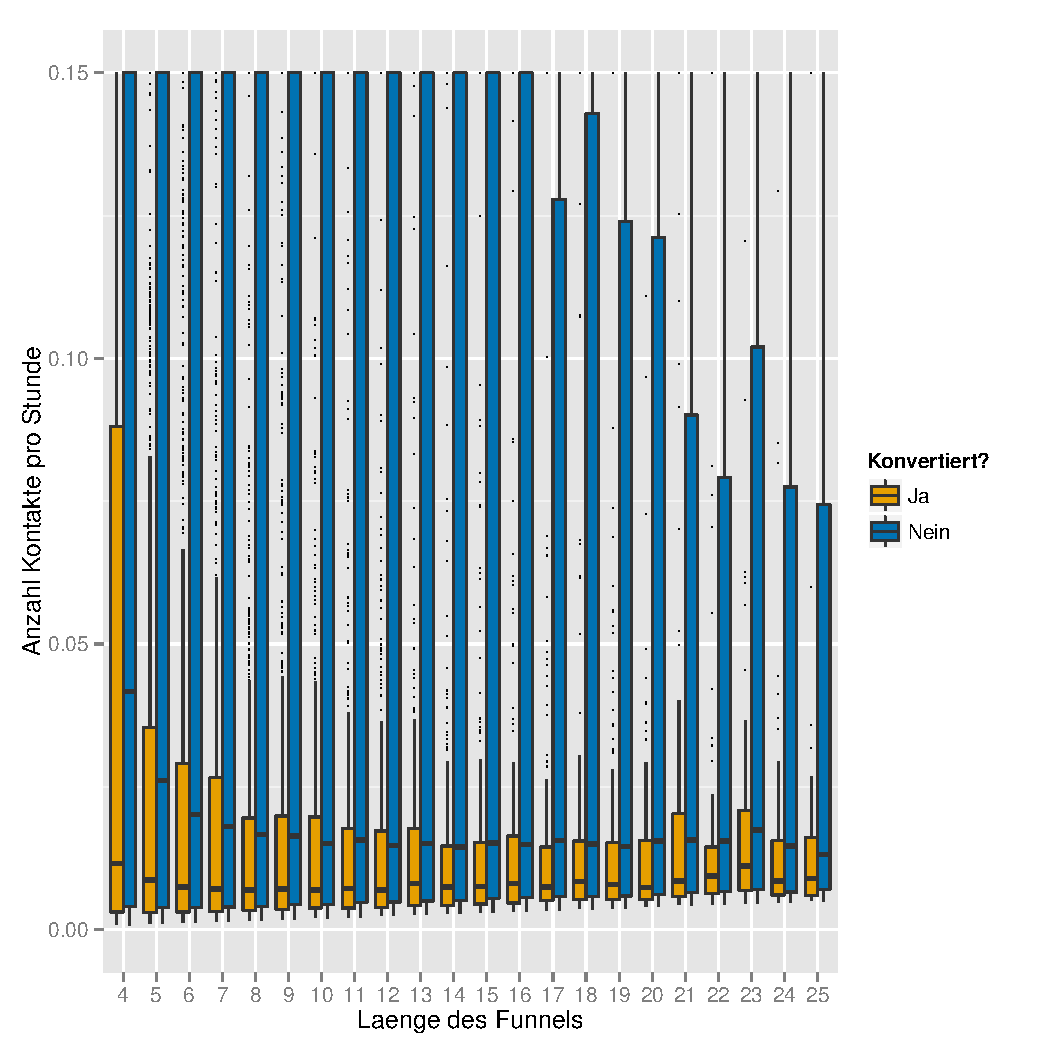
\includegraphics[scale=0.6]{freq.pdf}
	\caption[Frequenz der Kontaktpunkte]{Frequenz der Kontaktpunkte in konvertierten und nicht-konvertierten Funnels}
	\label{freq}
\end{figure}

\section{Zeitdiskretes Survival-Modell}\label{survival}

\subsection{Lebensdauer-Modell}\label{secModel1}

Aufgrund der in Kapitel \ref{datenlage} beschriebenen Datenlage erscheint die Anwendung eines Modells aus dem Feld der Lebensdaueranalyse intuitiv. Es wird die Zeit bis zu einem Ereignis betrachtet, welches in diesem Fall das Ausfüllen eines Online-Antrages ist. Der Kunde befindet sich während der Beobachtungsspanne im transienten Zustand bis er durch die Konvertierung in den absorbierenden Zustand wechselt, an dem die Beobachtung endet. Tritt am Ende der Beobachtung eines Kunden keine Konvertierung ein, so spricht man von einer Rechtszensierung.\\
Die Position gibt die Nummer des Kontaktpunktes an und bildet die Zeitachse des Modells. Das heißt, es handelt sich um ein zeitdiskretes Modell und die Zielvariable $y_{ip}$ (\ref{zielvar}) nimmt den Wert Eins an, wenn Kunde $i$ an der Position $p$ konvertiert ist. Für alle vorherigen Positionen eines konvertierten Funnels und für alle Positionen eines Nicht-konvertierten Funnels nimmt $y_{ip}$ den Wert Null an. $N_p$ ist die Anzahl der Beobachtungen an Position $p$. Diese nimmt mit steigendem $p$ ab, da in jeder Position Funnels konvertieren oder Beobachtungen ohne Konvertierung enden. Deshalb wird das Modell nur auf die ersten $25$ Positionen angewendet, da für spätere Positionen nicht ausreichend konvertierte Funnels vorliegen.\\
\begin{align}
	y_{ip} = \begin{cases} 1 & \text{Beobachtung } i \text{ konvertiert an Position } p\\
												 0 & \text{sonst} 
					 \end{cases} \text{, } p=1,...,25 \text{, } i=1,...,N_p \label{zielvar}
\end{align}
Das Modell schätzt die Hazardrate $\lambda_{ip}$ (\ref{haz}), das heißt die Wahrscheinlichkeit, dass Beobachtung $i$ an Position $p$ konvertiert unter der Bedingung, dass die Länge des Funnels von Beobachtung $i$ größer oder gleich $p$ ist, was lediglich bedeutet, dass für Beobachtung $i$ an Position $p$ überhaupt noch ein Kontaktpunkt vorliegt. Außerdem wird auf die Features $x_{ip}$ bedingt, die später noch näher erläutert werden.
\begin{align}
	\lambda_{ip} = P(y_{ip}=1|funnelLength_i \geq p, x_{ip}) \label{haz}
\end{align}
Die Hazardrate wird mittels eines Logit-Modells (\ref{logit1}-\ref{logit2}) mit der Zielvariable $y_{ip}$ an jeder Position $p$ seperat geschätzt. Die Annahmen des Modells sind, dass die $y_{ip}|x_{ip}$ unabhängig Bernoulli-verteilt sind mit der Hazardrate $\lambda_{ip}$ als Parameter und der Erwartungswert wird anhand der Responsefunktion $h$ mit der Prädiktorfunktion $f_{ip}$ verknüpft.
\begin{align}
	y_{ip}|x_{ip} &\stackrel{ind}{\sim} Bin(1, \lambda_{ip}) \label{logit1} \\
	E(y_{ip}|x_{ip}) = P(y_{ip} = 1|x_{ip}) = \lambda_{ip} &= h(f_{ip}) = \frac{\exp(f_{ip})}{1+\exp(f_{ip})}\label{logit2}
\end{align}
Aus diesen Annahmen lässt sich die Likelihood (\ref{lik}) und die Log-Likelihood (\ref{loglik}) des Modells ableiten.
\begin{align}
	L(\lambda_{ip}) &= \prod_{i=1}^{N_p} \lambda_{ip}^{y_{ip}} (1-\lambda_{ip})^{1-y_{ip}} \label{lik} \\
	l(\lambda_{ip}) &= \ln(L(\lambda_{ip})) = \sum_{i=1}^{N_p} (y_{ip} \ln(\lambda_{ip}) + (1-y_{ip}) \ln(1-\lambda_{ip})) \notag \\
	&= \sum_{i=1}^{N_p} (y_{ip} f(x_{ip}) - \ln(1+\exp(f(x_{ip})))) \label{loglik}
\end{align}
Damit ergibt sich der binomielle Verlust aus der negativen Log-Likelihood (\ref{binVer}) und das Logit-Modell ist lösbar durch die Minimierung dieses Verlusts (\ref{loes}).
\begin{align}
	L(y,f) = -yf + \ln(1+\exp(f)) \label{binVer} \\
	\argmin_{\beta_p} \sum_{i=1}^{N_p} L(y_{ip},f(x_{ip})) \label{loes}
\end{align}
Um ein gutes Prognose-Modell zu entwickeln, wird eine Ensemble-Methode angewendet, die im nächsten Abschnitt vorgestellt wird.

\subsection{Stochastic Gradient Boosting}\label{secModel2}

\subsubsection*{Algorithmus}

Stochastic Gradient Boosting ist eine Ensemble-Methoden, die durch mehrfache Anwendung des sogenannten Basis-Lerners ein Ensemble von Schätzern für eine Prognosefunktion liefert. Durch Aggregation der Schätzer erhält man die endgültige Prognosefunktion. Ein sehr beliebter Basis-Lerner sind Stümpfe, das heißt Bäume mit nur einem Split. Einige Vorteile von Bäumen sind, dass sie mit kategoriellen Features, Ausreißern und fehlenden Werten umgehen können. Außerdem wird der schwachen Prognoseleistung von Bäumen durch die Kombination mit Boosting entgegen gewirkt.\\
Gesucht ist also eine Prognosefunktion, die den Erwartungswert einer Verlustfunktion minimiert. Als Verlustfunktion wird der binomielle Verlust (\ref{binVer}) verwendet, wobei sich die Prädiktorfunktion wie folgt ergibt.
\begin{align}
	f(x_{ip}) =& \text{offset}(\hat{\lambda}_{i,p-1}) + \notag \\
						 &f_{weekday,p}(\text{weekday}_{ip}) + \notag \\
						 &f_{hour,p}(\text{hour}_{ip}) + \notag \\
						 &f_{campaign,p}(\text{campaign}_{ip}) + \notag \\
						 &f_{campaignLast,p}(\text{campaign}_{i,p-1}) + \notag \\
						 &f_{campaignLast2,p}(\text{campaign}_{i,p-2}) + \notag \\
						 &f_{timeSinceLast,p}(\text{timeSinceLast}_{ip}) + \notag \\
						 &f_{timeSinceFirst,p}(\text{timeSinceFirst}_{ip}) \label{praediktor}
\end{align}
Der Prädiktor ist also eine additive Funktion von Treppenfunktionen der sieben verwendeten Features und einem offset. Hier sei nochmal darauf hingewiesen, dass Features wie \textit{hasClicked} oder \textit{clickCount} nicht verwendet werden können, da die Views aufgrund der Problematik der Datenerhebung nicht berücksichtigt werden. Die verwendeten Einflussgrößen sind also der Wochentag und die Stunde des jeweiligen Kontaktpunktes, die Art des aktuellen und der letzten zwei Kontakte, sowie die Dauer seit dem vorherigen Kontakt und die Gesamtdauer seit dem ersten bis zum jetzigen Kontakt. Die Funktionen $f_{.,p}$ können theoretisch für verschiedene Positionen komplett unterschiedliche Formen annehmen. Es sei ausdrücklich darauf hingewiesen, dass $f_{campaignLast,p}(\textit{campaign}_{i,p-1})$ und $f_{campaign,p-1}(\textit{campaign}_{i,p-1})$ zwei unterschiedliche Funktionen sind. Erstere gibt den Einfluss der Art des vorherigen Kontaktpunktes auf die Konvertierungswahrscheinlichkeit an der Position $p$ wieder und zweitere den Einfluss der Art des aktuellen Kontaktpunktes auf die Konvertierungswahrscheinlichkeit an der Position $p-1$. Unter der Annahme, dass der Einfluss der Features an den verschiedenen Positionen ähnlich ist, fließt zusätzlich noch die Vorhersage des Modells der vorherigen Position als offset mit ein. Dadurch konnten die Ergebnisse besonders an späteren Positionen, an denen weniger Daten vorhanden sind, deutlich verbessert werden. Ergebnisse ohne offset sind im elektronischen Anhang zu finden.\\
Der offset fällt für Position eins weg, da es noch keine Vorhersagen eines vorherigen Modells gibt. Außerdem sind für Position eins die Features \textit{campaignLast}, \textit{campaignLast2}, \textit{timeSinceLast} und \textit{timeSinceFirst} offentsichtlich noch nicht vorhanden, so dass diese ebenfalls wegfallen. An Position zwei ist \textit{campaignLast2} noch nicht vorhanden und \textit{timeSinceLast} und \textit{timeSinceFirst} sind hier identisch, so dass nur eine der beiden berücksichtigt wird. Ab Position Drei ergibt sich der Prädiktor dann exakt so wie in (\ref{praediktor}) dargestellt.\\
\floatname{algorithm}{Algorithmus}
\begin{algorithm}
\caption{Gradient Boosting}\label{alg}
\label{gradboosting}
\begin{algorithmic}
\STATE Setze Startwert für $f_{0p}(x_{ip})$
\FOR{$m=1:n.trees$}
	\STATE Setzte $\lambda_{ip}(x_{ip}) = \frac{\exp(f_{m-1,p}(x_{ip}))}{1+\exp(f_{m-1,p}(x_{ip}))}$
	\FOR{$i=1:N_p$} 
		\STATE $r_{imp} = - \frac{\partial L(y_{ip},f_{m-1,p}(x_{ip}))}{\partial f_{m-1,p}(x_{ip})} = y_{ip} - \lambda_{ip}(x_{ip})$
	\ENDFOR
	%\STATE Fit a regression base learner to the pseudo-residuals $r_{im}$:
	\STATE $\theta_{mp} = \argmin_{\theta} \sum_{i=1}^{N_p} (r_{imp} - h(x_{ip}, \theta))^2$
	\STATE $\beta_{mp} = \argmin_{\beta} \sum_{i=1}^{N_p} L(y_{ip}, f_{m-1,p}(x_{ip}) + \beta h(x_{ip},\theta_{mp}))$
	\STATE $f_{mp}(x_{ip}) = f_{m-1,p}(x_{ip}) + \beta_{mp} h(x_{ip},\theta_{mp})$
\ENDFOR
\end{algorithmic}
\end{algorithm}
Algorithmus \ref{alg} enthält Pseudo-Code, der das Vorgehen beim Gradient Boosting erläutern soll. Dieser muss für jedes $p=1,...,25$ durchgeführt werden. Zunächst muss ein Startwert des Prädiktors $f_{0p}$ festgelegt werden. Daraufhin werden folgende Schritte für $m=1$ bis \textit{n.trees} iteriert. Für jede Beobachtung $i$ werden die Pseudo-Residuen $r_{imp}$ berechnet, die die Richtung des negativen Gradienten angeben. Die Pseudo-Residuen entsprechen also der Richtung des steilsten Abstiegs der Verlustfunktion. An die Pseudo-Residuen wird ein Basis-Lerner $h(x_{ip},\theta_{mp})$, in diesem Fall ein Entscheidungsbaum, so angepasst, dass er den negativen Gradienten so gut wie möglich approximiert. Bildlich gesprochen wird das Modell also in die Richtung der größten Verringerung des Verlusts verschoben. Da als Basis-Lerner Stümpfe verwendet werden, wird die Verbesserung des Modells in einem Boosting-Schritt durch nur eines der sieben Features erklärt. Per Line-Search wird daraufhin die optimale Schrittweite $\beta_{mp}$ berechnet und das Modell wird geupdatet mit $f_{mp}(x_{ip}) = f_{m-1,p}(x_{ip}) + \beta_{mp} h(x_{ip},\theta_{mp})$. Nach \textit{n.trees} Iterationen endet der Algorithmus.\\
Durch die Verringerung des Verlusts in jeder Iteration kann es vor allem bei einer hohen Anzahl von Iterationen zu Overfitting kommen. Deshalb wird mittels Kreuzvalidierung die optimale Anzahl an Iterationen ausgewählt. Das heißt $\hat{f}(x_{ip}) = f_{m\_opt,p}(x_{ip})$ wird als Ergebnis verwendet. Das Ensemble der Splits bildet für jedes der Feautures eine Treppenfunktion.

\subsubsection*{Parameter des Modells}

Das Modell wurde mit dem Paket \textit{gbm} \cite{gbm} in \textit{R} \cite{r} berechnet und mit Hilfe der R-Pakete \textit{foreach} \cite{foreach} und \textit{doSNOW} \cite{dosnow} parallelisiert. Die Modelle für die einzelnen Positionen können allerdings nur dann parallelisiert werden, wenn kein offset benützt wird. Für die Anwendung des Modells müssen noch einige Parameter eingestellt werden.\\
Zunächst wurden die Daten in Trainings- und Testdaten aufgeteilt, sodass Trainings- und Testdaten jeweils die Hälfte der gesamten Daten ausmachen. Da die Anzahl der nicht-konvertierten Funnels deutlich überwiegt und einige Kampagnen vergleichsweise selten in den Daten auftreten, wurden die Trainingsdaten stratifiziert bezüglich konvertierter beziehungsweise nicht-konvertierter Funnel und der Variable \textit{Campaign} gezogen. Außerdem wurde die Länger der Funnels berücksichtigt, so dass  Trainings- und Testdaten positionsübergreifen klar getrennt sind und das Verhältnis von eins zu eins trotzdem eingehalten wird. Das heißt, dass ein Beobachtung, die an Position $1$ in den Trainingsdaten enthalten ist auch an allen späteren Positionen in den Trainingsdaten ist. Das selbe gilt für die Testdaten. Dies ist wichtig, damit Trainings- und Testdaten bei der Anwendung des offsets nicht vermischt werden. Anhand der Trainingsdaten wurde das Modell gefittet. Die Testdaten dienen der späteren Bewertung der Prognosegüte des Modells. Die maximale Anzahl der Bäume \textit{n.trees} wurde gleich $3000$ gesetzt, wobei für die Präsentation der Ergebnisse die optimale Anzahl an Bäumen mittels 5-facher Kreuzvalidierung gewählt wurde.\\
Zusätzlich zu der Beschränkung der Iterationen, wird dem Overfitting auch durch einen Shrinkage-Parameter $\mu$ entgegen gewirkt. Dieser bewirkt, dass nicht die optimale Schrittweite $\beta_{mp}$ in jeder Iteration gegangen wird, sondern nur ein Bruchteil dieser Schrittweite. Es wird also durch $f_{mp}(x_{ip}) = f_{m-1,p}(x_{ip}) + \mu \beta_{mp} h(x_{ip},\theta_{mp})$ geupdatet, wobei $\mu$ gleich $0.01$ gewählt wurde, was einem üblichen Wert für diesen Parameter entspricht. Bei der Wahl von $\mu$ und \textit{n.trees} muss stets die Rechenzeit im Auge behalten werden.\\
Wie bereits erwähnt, wurden als Basis-Lerner Stümpfe gewählt. Das wurde durch die Festlegung von \textit{interaction.depth} auf $1$ realisiert. Mit einer höheren \textit{interaction.depth} ließen sich auch Interaktionen modellieren. Die Stärke von solchen Interaktionen lassen sich beispielsweise mit Friedmans h-Statistik \cite{friedman_h} untersuchen. Die Einführung von Interaktionen führt bei den vorliegenden Daten aber zu einer drastischen Verschlechterung der Prognosegüte und schwer interpretierbaren Ergebnissen. Bei Interesse sind Ergebnisse diesbezüglich im elektronischen Anhang zu finden.\\
Der bis hierhin beschriebene Algorithmus entspricht lediglich dem Gradient Boosting. Wenn man in jeder Iteration allerdings nur einen Teil der Daten verwendet, spricht man vom Stochastic Gradient Boosting. Diese Anpassung führt meist zur einer Verbesserung der Ergebnisse \cite{fried_additive}, wobei noch nicht geklärt ist, wie genau es zu dieser Verbesserung kommt. In diesem Modell wurde die \textit{bag.fraction}, das heißt der Anteil der verwendeten Daten in jedem Schritt, auf $0.5$ gesetzt.

\subsubsection*{Output}

Als Ergebnis ist für jede Beobachtung $i$ und jede Position $p$ ein Wert $\hat{f}(x_{ip})$ gegeben. Daraus können die Hazardraten durch Rücktransformation (\ref{trafo}) berechnet werden.
\begin{align}
	\hat{\lambda}_{ip} = \frac{\exp(\hat{f}(x_{ip}))}{1+\exp(\hat{f}(x_{ip}))} \label{trafo}
\end{align}
Diese geben die Wahrscheinlichkeit für Beobachtung $i$ an Position $p$ zu konvertieren an. Da die nicht-konvertierten Funnels in den Daten deutlich überwiegen, sind diese Wahrscheinlichkeiten sowohl für konvertierte als auch für nicht-konvertierte Funnels sehr niedrig. Deshalb kommt der Bayes-Klassifikator zur Beurteilung der Prognosegüte nicht in Frage, da dieser schlicht alle Beobachtungen als nicht konvertiert vorhersagen würde.\\
Es muss also ein geeigneter Schwellenwert gefunden werden, um die Prognosegüte des Modells zu bewerten. Wenn die Hazardrate einer Beobachtung größer ist als der Schwellenwert, so wird diese als konvertiert vorhergesagt und sonst als nicht-konvertiert. Dafür werden die Kenngrößen Sensitivität und Spezifität benötigt. Die Sensitivität ist die Richtig Positiv Rate, das heißt der Anteil der wirklich Konvertierten unter allen, die als konvertiert vorhergesagt werden, gegeben ein spezifischer Schwellenwert. Die Spezifität ist die Richtig Negativ Rate, das heißt der Anteil der Nicht-Konvertierten unter allen, die als nicht-konvertiert vorhergesagt werden. Diese Kennwerte wurden für ein Gitter von potentiellen Schwellenwerten berechnet.\\
Die ROC (Receiver Operating Characteristics)-Kurve erlaubt die simultane Betrachtung dieser Schwellenwerte. Diese bildet die Falsch Positiv Rate, das heißt $1$ minus Spezifität, auf der x-Achse und die Sensitivität auf der y-Achse ab. Die ROC-Kurve hat ihren Ursprung im Punkt $(0,0)$ und steigt von dort monoton an bis $(1,1)$. Wenn Falsch Positiv Rate und Richtig Positiv Rate für alle Schwellenwerte gleich ist, so kann das Modell nicht zwischen konvertiert und nicht-konvertiert unterscheiden und die ROC-Kurve ist die Diagonale zwischen $(0,0)$ und $(1,1)$. Ein perfektes Modell, dass alle Beobachtungen korrekt zuweist geht durch den Punkt $(0,1)$. Je größer die Fläche zwischen der Diagonalen und der ROC-Kurve ist, desto besser ist somit auch das Modell.\\
An dieser Stelle kommt die AUC (Area Under the Curve) ins Spiel. Sie ist definiert als die Fläche unter der ROC-Kurve (\ref{formelAUC}). Wenn das Modell nicht zwischen konvertiert und nicht-konvertiert unterscheiden kann, so ist die AUC gleich $0.5$ und die ROC ist, wie bereits erwähnt die Diagonale. Ein AUC von $1$ entspricht einem perfekten Modell. Die AUC wird interpretiert als die Wahrscheinlichkeit, dass bei einer konvertierten Beobachtung die Hazardrate größer ist als bei einer nicht-konvertierten Beobachtung.
\begin{align}
	AUC = \int_0^1 \! ROC(t) \, \mathrm{d}t. \label{formelAUC}
\end{align}
Ein weiterer Kennwert, der die Prognosefunktion beschreibt, ist die Relative Wichtigkeit der Einflussgrößen \cite{fried_greedy}. Sie gibt die Stärke des Einflusses der Features auf die Prognoseregel an. $\hat{I}_{jp}^2(m)$ (\ref{rel1}) ist die Verbesserung, die an Position $p$ in Iteration $m$ durch die Variable $j$ realisiert wird, wobei $\hat{i}_{mp} 1_{jmp}$ eben diese Verbesserung ist und $1_{jmp}$ die Indikatorfunktion, die angibt, ob in Iteration $m$ das Feature $j$ als Splitvariable genutzt wurde. $\hat{I}_{jp}^2$ (\ref{rel2}) mittelt für jedes Feature $j$ über alle Iterationen beziehungsweise Bäume und die Relative Wichtigkeit $\hat{I}_{jp}$ (\ref{rel3}) von Feature $j$ ergibt sich dann aus der Wurzel dieses Wertes. Die Wichtigkeitswerte werden so skaliert, dass sie in der Summe den Wert $100$ ergeben.
\begin{align}
	\hat{I}_{jp}^2(m) &= \hat{i}_{mp} 1_{jmp} \label{rel1} \\
	\hat{I}_{jp}^2 &= \frac{1}{M} \sum_{m=1}^{n.trees} \hat{I}_{jp}^2(m) \label{rel2} \\
	\hat{I}_{jp} &= \sqrt{\hat{I}_{jp}^2} \label{rel3}
\end{align}
Neben der Information zur Stärke des Einflusses eines Features, interessiert natürlich auch die Art dieses Einflusses, das heißt der marginale Effekt eines Features \cite{fried_greedy}. Das Ziel ist somit ein Plot, der den Zusammenhang zwischen dem Feature $j$ und der Prognosefunktion $\hat{f}$ an Position $p$ darstellt. Da die Prognosefunktion von mehreren Features abhängt, müssen die marginalen Effekte berechnet werden. Das Feature $x_{jp}$ ist eine Teilmenge aller Features $\{x_{1p},...,x_{np}\}$ und $x_{\backslash j,p}$ sei dessen Komplement. Damit kann die Prognosefunktion als $\hat{f}(x_p)=\hat{f}(x_{jp},x_{\backslash j,p})$ geschrieben werden und wenn man auf bestimmte Werte von $x_{\backslash j,p}$ bedingt, kann die Prognosefunktion als Funktion von lediglich $x_{jp}$ betrachtet werden.
\begin{align}
	\hat{f}_{x_{\backslash j,p}}(x_{jp}) = \hat{f}(x_{jp}|x_{\backslash j,p})
\end{align}
Die Form von $\hat{f}_{x_{\backslash j,p}}(x_{jp})$ hängt von dem für $x_{\backslash j,p}$ gewählten Wert ab. Wenn diese Abhängigkeit nicht zu stark ist, dann ist (\ref{marg}) eine gute Zusammenfassung des marginalen Effektes von $x_{jp}$ auf die Prognosefunktion. Dabei ist $p_{\backslash j,p}(x_{\backslash j,p})$ die marginale Dichte von $x_{\backslash j,p}$ und $p(x_p)$ ist die gemeinsame Dichte der Features.
\begin{align}
	\bar{f}_{jp}(x_{jp}) = E_{x_{\backslash j,p}}(\hat{f}(x_p)) = \int \! \hat{f}(x_{jp},x_{\backslash j,p}) p_{\backslash j,p}(x_{\backslash j,p}) \, \mathrm{d}x_{\backslash j,p}. \label{marg} \\
	p_{\backslash j,p}(x_{\backslash j,p}) = \int \! p(x_p) \, \mathrm{d}x_{\backslash j,p}.
\end{align}
Die marginale Dichte kann aus den Trainingsdaten geschätzt werden, so dass (\ref{marg}) zu (\ref{marg1}) wird.
\begin{align}
	\bar{f}_{jp}(x_{jp}) = \frac{1}{N} \sum_{i=1}^{N_p} \hat{f}(x_{jp},x_{i,\backslash j,p}) \label{marg1}
\end{align}
Die marginalen Effekte werden wiederum zu den Hazardraten rücktransformiert.

\section{Sequential Pattern Mining}\label{spm}

\subsection{Überblick}

\textit{Sequential pattern mining} entdeckt häufige \textit{subsequences} (dt. Teilfolgen) in Datenbanken. Sogenannte \textit{sequence databases} bestehen aus Transaktionen, die jeweils \textit{items} enthalten, welche der Zeit nach geordnet sind. Die Daten lassen sich also mit dem Schema [Transaction/ID, <Ordered Sequence Items>] darstellen.\\
Ein Anwendungsfeld ist die Warenkorbanalyse. Angenommen es wird das Kaufverhalten in einem Supermarkt einen Monat lang beobachtet, dann könnte [Kunde 1, <(Brot, Milch), (Brot, Milch, Tee), (Zucker), (Milch, Salz)>]; [Kunde 2, <(Brot), (Milch, Tee)>] eine Beispiel-Datenbank sein. Kunde 1 war vier mal im beobachteten Monat im Supermarkt einkaufen, wobei Kunde 2 nur zweimal einkaufen war. Der Kunde kann nur eins oder auch mehrere \textit{items} pro Besuch einkaufen. Im Falle von mehreren \textit{items} spricht man von \textit{itemsets}.\\
\textit{Web usage mining} ist das am weitesten verbreitete Anwendungsfeld von \textit{sequential pattern mining} in der Literatur (\cite{lu_ezeife,wang_han,goethals}). Unter der Annahme, dass ein Internetnutzer nur eine Webseite an einem Zeitpunkt aufrufen kann, besteht die Folge von geordneten \textit{items} nur aus einzelnen \textit{items} und nicht aus \textit{itemsets}. Ist also eine Menge von \textit{items I = \{a, b, c, d, e\}} gegeben, die beispielsweise verschiedene Webseiten repräsentieren, so könnte eine Datenbank mit zwei Nutzern folgendermaßen aussehen: [Nutzer 1, <abedcab>]; [Nutzer 2, <edcaa>] (\cite[3:1-3:2]{taxonomy}).

\subsection{Notationen und Definitionen}
Gegeben ist eine Menge von Sequenzen, die eine sequentielle Datenbank $D$ bilden, ein minimum support threshold $min\_sup$ $\xi$ und eine Menge von $k$ eindeutigen items $I=\{i_1,i_2,...,i_k\}$. Das Ziel von sequential pattern mining ist das Finden aller häufig auftretenden Sequenzen $S$ von items aus $I$ in der Datenbank $D$ bei gegebenem $min\_sup$ $\xi$.\\
Im vorliegenden Fall sind die items die verschiedenen Marketing-Kanäle, die hier beispielhaft als $I=\{a,b,c,d,e\}$ dargestellt sind. Ein itemset ist eine nichtleere, ungeordnete Menge von items, zum Beispiel $(eab)$. Lexikographisch geordnete itemsets bilden eine Sequenz, beispielsweise $S=<b(eab)ac(cd)>$.\\
Set Lexicographical Order (\cite{lexico}) kann wie folgt definiert werden. Gegeben ein itemset $t=\{i_1,i_2,...,i_k\}$ mit $k$ unterschiedlichen items und ein weiteres itemset $t'=\{j_1,j_2,...,j_l\}$ mit $l$ unterschiedlichen items mit $i_1\le i_2\le ...\le i_k$ und $j_1\le j_2\le ... \le j_l$, wobei $i_1\le i_2$ bedeutet, dass $i_1$ vor $i_2$ eintritt. Dann gilt $t<t'$, wenn (1) für $h\in\mathbb{N}$, $0\le h\le min\{k,l\}$, $r<h$ und $i_h<j_h$ gilt $i_r=j_r$ oder (2) $k<l$ und $i_1=j_1$, $i_2=j_2,...,i_k=j_k$.\\
Eine Sequenz $\alpha=<\alpha_1\alpha_2...\alpha_m>$ ist Subsequenz einer anderen Sequenz $\beta=<\beta_1\beta_2...\beta_n>$, in Zeichen $\alpha\preceq\beta$, wenn eine injektive, isotone Funktion $f$ existiert, die items in $\alpha$ auf items in $\beta$ abbildet, das heißt (1) $\alpha_i\subseteq f(\alpha_i)$ und (2) wenn $\alpha_i<\alpha_j$ ist, dann ist $f(\alpha_i)<f(\alpha_j)$.


\subsection{Auswahl geeigneter Algorithmen}

In den letzten zwei Jahrzehnten wurden im Forschungsfeld des \textit{sequential pattern mining} eine Vielzahl von Algorithmen entwickelt (\cite{hvsm,lapin,aprioriall,gsp,psp,spam,freespan,prefixspan,wapmine,fsminer,discall,spade,plwap}; \textbf{die die an anderer stelle zitiert werden, hier später löschen}). Im Folgenden sollen die besten Algorithmen für die gegebene Datenlage ausgewählt werden.

\section{Visualisierung der Daten anhand eines Netzwerkes}\label{network}

Während Sequential Pattern Mining lediglich häufige Sequenzen in den Daten findet, sollen die Daten zusätzlich noch in Form eines Netzwerkes dargestellt werden. Dies ermöglicht die Visualisierung des kompletten Datensatzes und liefert weitere Informationen bezüglich von Mustern in den Daten.\\
Zum bessern Verständnis sollen an dieser Stelle einige elementare Grundlagen der Graphentheorie vorgestellt werden. Ein geordneter Graph $G=(V,E)$ besteht aus einer Menge $V$ von Knoten und einer Menge $E$ von Kanten. Eine Kante $e_i \in E$ besteht aus einem geordneten Paar von zwei Knoten $(v_j,v_k)$, wobei $v_j,v_k \in V$. Das heißt eine Kante stellt die geordnete Verbindung zwischen zwei Knoten dar \cite[16]{network_data}.\\
Das Netzwerk ist wie folgt strukturiert. Ausgehend von einem Startpunkt führen $17$ Kanten zu den $17$ Kampagnen der ersten Position. Diese $17$ Kampagnen entsprechen jeweils einem Knoten. Die Namen der Knoten setzen sich aus dem Namen der Kampagne und $\_1$ für Position $1$ zusammen. Von jeder Kampagne führt dann eine Kante zu $Success\_1$ für die Funnels, die nach einem Kontakt konvertiert sind sowie eine Kante zu $Fail\_1$ für die Funnels, deren Beobachtung nach einem Konaktpunkt ohne Konvertierung abbricht. Außerdem führen von jeder der $17$ Kampagnen der ersten Position jeweils $17$ Kanten zu den $17$ Kampagnen der zweiten Position. Die Knoten der zweiten Position setzen sich wiederum aus dem Namen der Kampagne und $\_2$ zusammen. Von dort führen wieder Kanten zu $Success\_2$, $Fail\_2$ und den Kampagnen der dritten Position. Dieses Prinzip setzt sich für die weiteren Positionen fort.\\
Diese Kanten werden bezüglich der Anzahl der Nutzer gewichtet. Anhand imaginärer Zahlen soll hier das Prinzip kurz dargestellt werden. Wenn $50000$ Nutzer als ersten Kontakt $Direct$ haben, so hat der Knoten $Direct\_1$ ein Gewicht von $50000$. Diese verteilen sich nun auf die Knoten, die mit $Direct\_1$ durch eine Kante verbunden sind. Wenn die Kante zwischen $Direct\_1$ und $Direct\_2$ beispielsweise ein Gewicht von $10000$ hat, so haben $10000$ Nutzer als ersten und zweiten Kontakt $Direct$. Wenn die Kante zwischen $Direct\_1$ und $Success\_1$ ein Gewicht von $500$ hat, so bedeutet das, dass $500$ Nutzer als ersten Kontakt $Direct$ haben und danach direkt konvertieren.\\
Um aussagekräftigere Ergebnisse zu erzielen, wurden für die Gewichtung der Kanten nicht die absoluten Anzahlen gewählt. Stattdessen wurden zwei Strategien verfolgt, die im folgenden als relative Ausgänge beziehungsweise relative Eingänge bezeichnet werden. Für die relativen Ausgänge werden die Kanten mit den relativen Häufigkeiten gewichtet, wobei die zugrundeliegende Menge die Summe aller Nutzer ist, die einen Knoten verlassen. Das heißt die Summe der Gewichte aller Kanten, die einen Knoten verlassen ergeben in der Summe $1$. Wenn nun das Gewicht der Kante zwischen $Direct\_2$ und $Fail\_2$ $0.2$ entspricht, so sind $20 \%$ der Nutzer, die als zweiten Kontakt $Direct$ haben, nach dem zweiten Kontaktpunkt konvertiert. Diese Gewichtung erlaubt somit eine relative Betrachtung der Kanten die eine Kampagne verlassen.\\
Für die relativen Eingänge werden die Kanten ebenfalls mit den relativen Häufigkeiten gewichtet, wobei die zugrundeliegende Menge nun die Summe aller Nutzer ist, die in einen Knoten gehen. Betrachtet man beispielsweise $Success\_2$, so kann man erkennen, aus welchen Kampagnen der zweiten Position sich die konvertierten Funnels der Länge $2$ zusammen setzen. Hat die Kante zwischen $Direct\_2$ und $Success\_2$ nun einen Gewicht von $0.2$, so haben $20 \%$ der konvertierten Funnels der Länge $2$ als letzten Kontaktpunkt vor der Konvertiertung $Direct$. Somit sind zwei verschiedene Interpretationsmöglichkeiten durch die unterschiedliche Gewichtung der Kanten gegeben.\\
Das Netzwerk mit den gewichteten Kanten wird in \textit{R} mit dem Paket \textit{rgexf} \cite{rgexf} erzeugt und als \textit{gexf}-Datei exportiert. Daraufhin wird die Datei in das Open-Source Programm \textit{Gephi} \cite{gephi_bastian} geladen. Dort werden die Daten dann als Graph dargestellt. Abbildung \ref{graphbegin} zeigt die räumliche Anordnung der Knoten und Kanten nach dem ersten Einlesen der \textit{gexf}-Datei in \textit{Gephi}, die noch willkürlich ist. Die farbigen Punkte sind die Knoten und die Linien die Kanten.\\
Für die Berechnung der räumlichen Anordnung der Knoten und Kanten stehen in \textit{Gephi} einige Algorithmen zur Verfügung. Diese berechnen die Anordung der Knoten anhand der Anziehungs- beziehungsweise Abstoßungskraft der Knoten, die aus den relativen Häufigkeiten resultieren. Stärker verbundene Knoten liegen damit näher beieinander als schwach verbundene. Das heißt Knoten, die überhaupt keine Verbindung enthalten, liegen weiter auseinander. Ein Beispiel wäre $Direct\_1$ und $Direct\_3$, da man von der ersten Position nicht direkt zur dritten Position springen kann, sondern zunächst einen Kontaktpunkt an der zweiten Position benötigt. Durch die Anwendung eines Algorithmus ergibt sich somit eine lineare Struktur, die die Positionen aneinander reiht.\\
Für diese Arbeit wurden der Algorithmus \textit{Force Atlas 2} \cite{forceatlas2} und der Algorithmus nach \textit{Yifan Hu} \cite{yifanhu} verwendet, wobei \textit{Yifan Hu} das Netzwerk besser in einzelne Ebenen einteilen kann. Das heißt die Positionen sind hier räumlich deutlicher getrennt. Für die Präsentation der Ergebnisse in Kapitel \ref{resultsnetwork} wurde die räumliche Anordnung der Knoten allerdings noch manuell bearbeitet, um die Ergebnisse anschaulicher zu machen.\\
\begin{figure}[H]
	\centering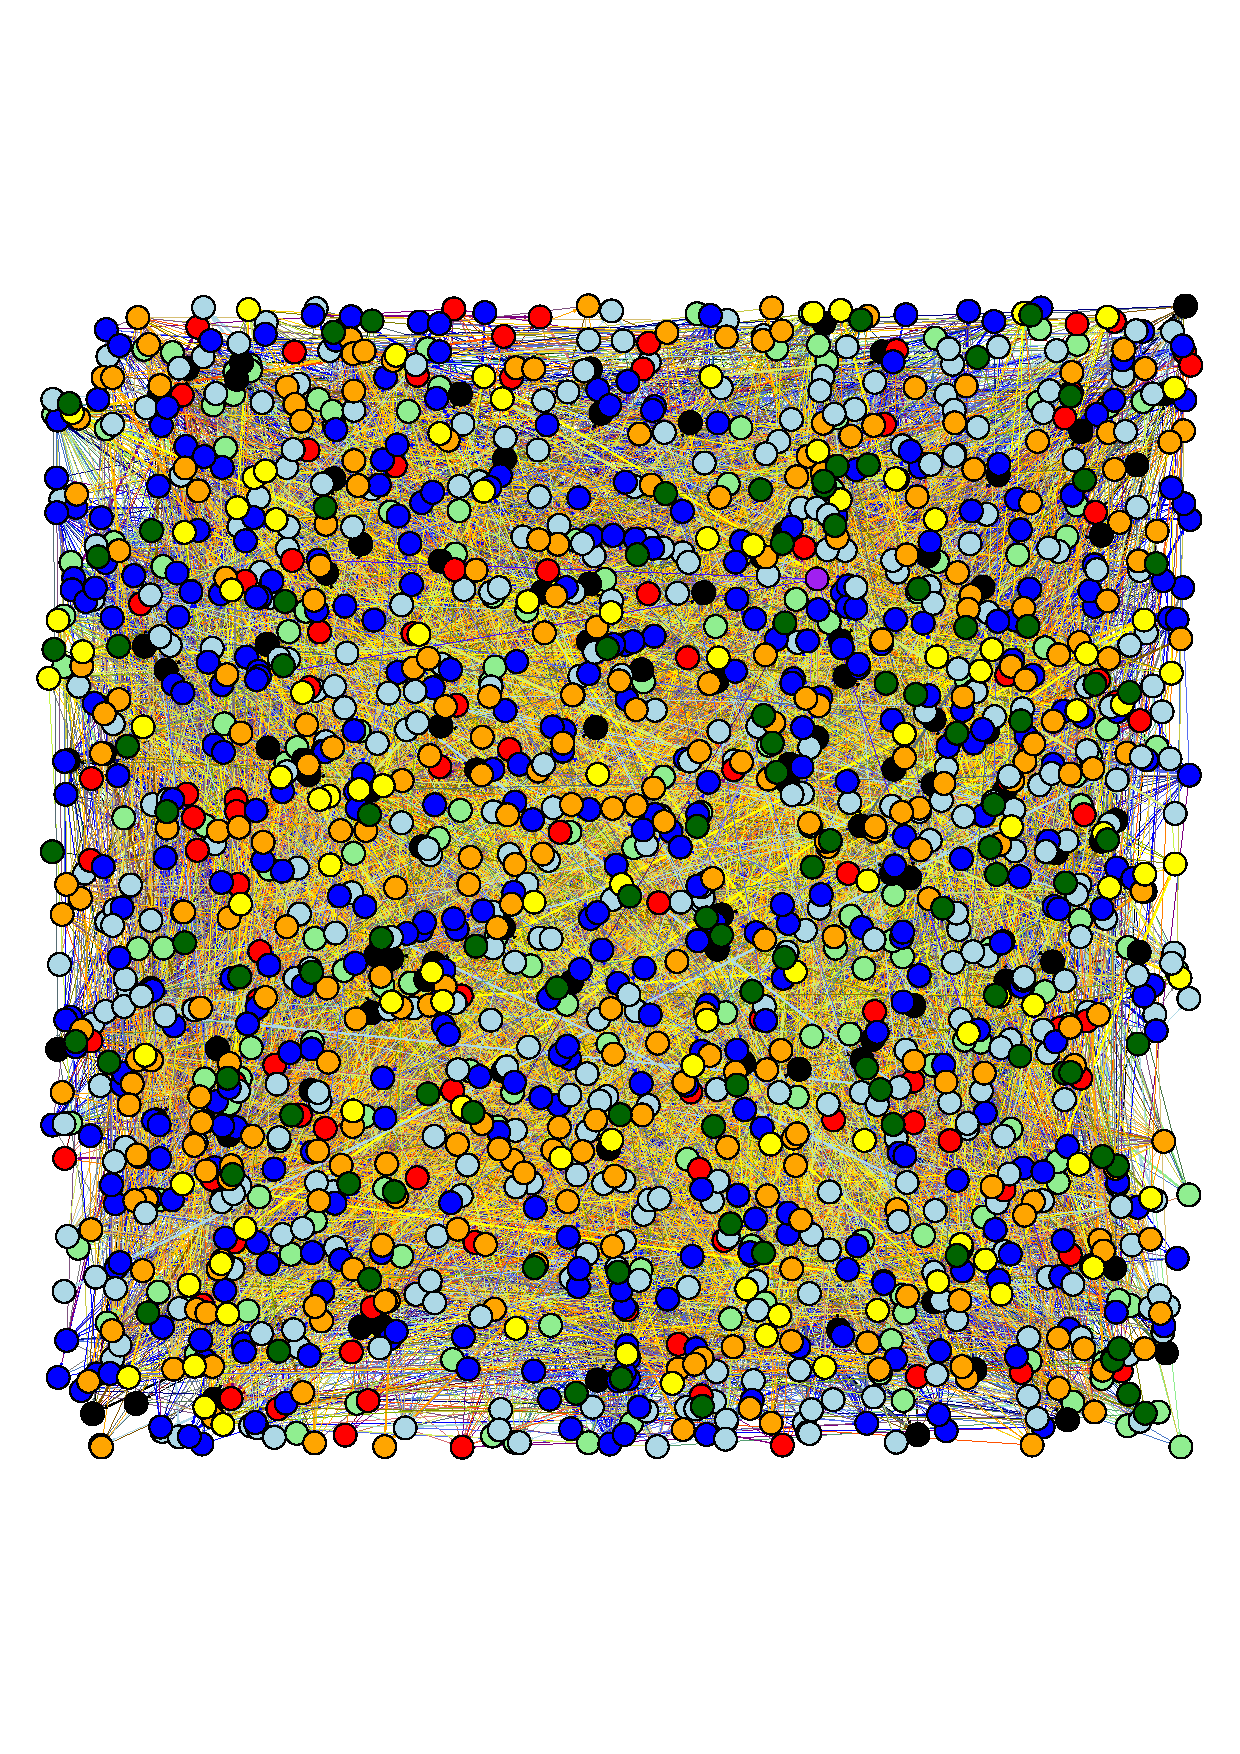
\includegraphics[scale=0.5]{graphbegin.pdf}\caption[Anordnung der Knoten nach dem Einlesen]{Anordnung der Knoten und Kanten direkt nach dem Einlesen in Gephi}\label{graphbegin}
\end{figure}
\noindent Das Netzwerk kann in \textit{Gephi} interaktiv bearbeitet werden. Die Daten sowie das Programm sind im elektronischen Anhang enthalten und werden in Kapitel \ref{anhang} näher beschrieben.




\section{Ergebnisse}\label{ergebnisse}

\subsection{Zeitdiskretes Survival-Modell}

Die in diesem Kapitel präsentierten Ergebnisse basieren jeweils auf der bestmöglichen Anzahl an Iterationen. Diese wurden mittels $5$-facher Kreuzvalidierung ermittelt und sind in Abbildung \ref{best_iter} dargestellt. Auf der $x$-Achse ist die Position von $1$ bis $25$ aufgetragen und auf der $y$-Achse die Optimale Iterationsanzahl, die durch $n.trees = 3000$ nach oben begrenzt ist. Es ist zu erkennen, dass für die Positionen $1$ bis $4$ über $2500$ Stümpfe für die Ergebnisse verwendet werden. Dann fällt die Kurve sehr schnell ab bis sie sich bei ungefähr $500$ Iterationen einpendelt. Dieser Abfall ist dadurch zu erklären, dass mit steigender Position die Datenmenge sinkt.\\
\begin{figure}[H]
	\centering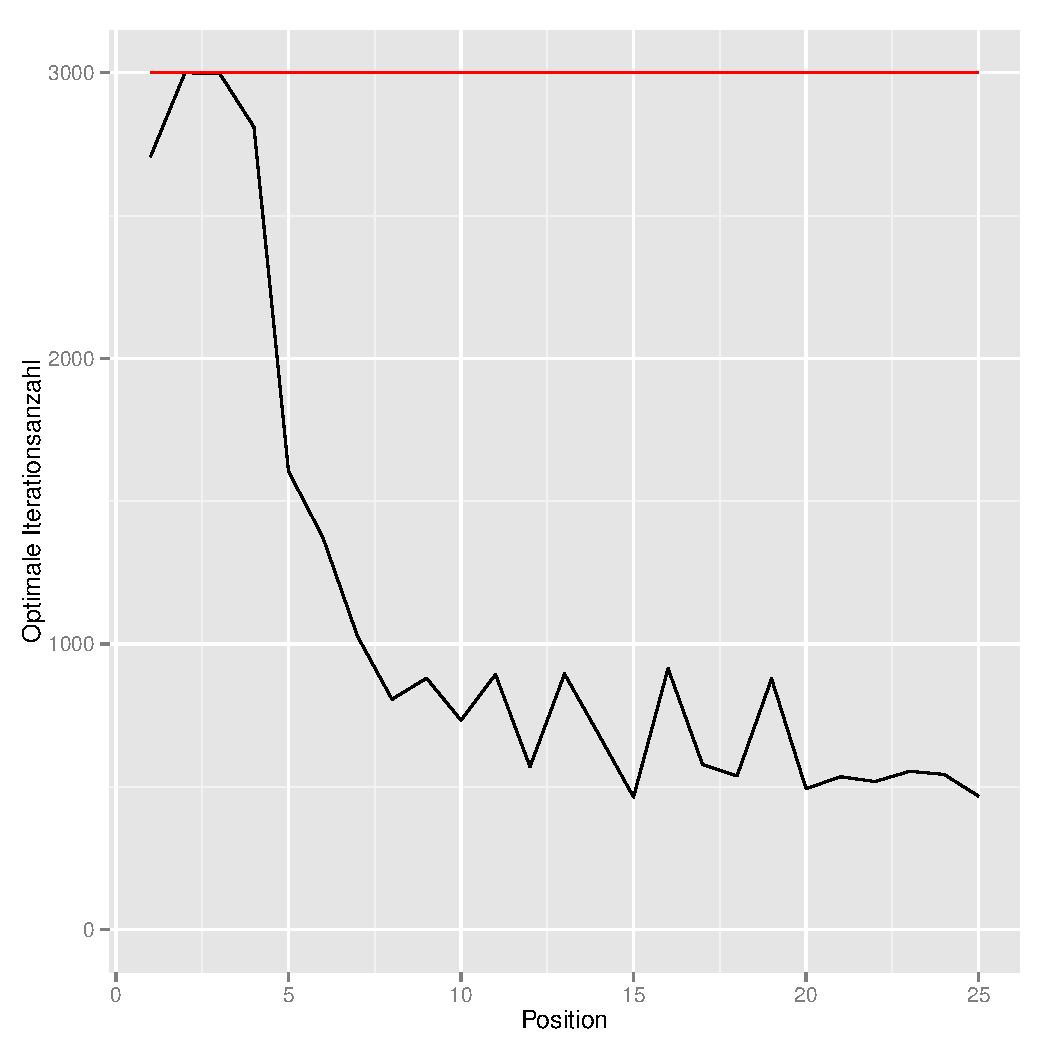
\includegraphics[scale=0.5]{bestIter.pdf}\caption[Optimale Iterationsanzahl]{Optimale Iterationsanzahl des Stochastic Gradient Boosting}\label{best_iter}
\end{figure}
\noindent Der relative Einfluss der Features gibt dessen Wichtigkeit bei der Erstellung der Prädiktorfunktion an und ist in Abbildung \ref{variable_importance} dargestellt. Auf der $x$-Achse ist erneut die Position aufgetragen und auf der $y$-Achse der relative Einfluss. Der relative Einfluss aller Features an einer Position ergibt summiert jeweils $100$ und die Balken sind der Größe nach geordnet, das heißt die wichtigsten Variablen sind unten abgebildet. Die Farben der Balken werden in der Legende rechts neben der Abbildung erläutert.\\
An Position $1$ sind nur drei Features vorhanden, wobei $Campaign$, das heißt die Art des Kontaktpunktes, für circa $90 \%$ der Minimierung der Verlustfunktion verantwortlich ist. Die Variablen $Hour$ und $Weekday$ haben kaum Einfluss. An Position $2$ ist die Kampagne immer noch das stärkste Feature, wobei hier auch die Kampagne des ersten Kontaktpunktes und die Zeit, die seit dem ersten Kontaktpunkt vergangen ist, Einfluss haben.\\
An den Positionen $8$ und $22$ hat die Kampagne des letzten Kontaktpunktes den stärksten Einfluss und damit selbstverständlich auch einen höheren Einfluss als die Kampagne des aktuellen Kontaktpunktes, die insbesondere an den höheren Positionen oft nur noch einen geringen Einfluss hat. Mit steigender Position wird auch die Kampagne des vorletzten Kontaktes wichtiger und ist manchmal das wichtigste Feature. Die Zeit, die seit dem vorherigen Kontaktpunkt vergangen ist, ist bereits an Position $3$ zweitwichtigstes Feature und spielt auch für die folgenden Positionen eine Rolle. Später nimmt die Wichtigkeit dieses Features allerdings ab und die Zeit, die seit dem ersten Kontaktpunkt vergangen ist, wird bedeutend wichtiger. Die Features $Hour$ und $Weekday$ spielen positionsübergreifend kaum eine Rolle.\\
Nachdem die Wichtigkeit der Variablen für die Klassifizierung in konvertierte und nicht-konvertierte Funnel präsentiert wurde, ist nun die Art dieses Einflusses interessant. Dieser wird im folgenden für einige Positionen dargestellt, wobei die Variablen dafür nach positionsspezifischer Wichtigkeit ausgesucht werden und das Augenmerk vor allem auf die niedrigeren Positionen fällt, da dort mehr Daten vorhanden sind. Folglich werden die Features $Hour$ und $Weekday$ garnicht präsentiert, das sie kaum einen Einfluss haben. Die Kampagne des vorletzten Kontaktpunktes $CampaignLast2$ wird an dieser Stelle ebenfalls nicht berücksichtigt, da die Ergebnisse für $Campaign$ beziehungsweise $CampaignLast$ oft sehr ähnlich sind. Im elektronischen Anhang sind die marginalen Effekte aller Features für jeweils jede Position zu finden.
\begin{figure}[H]
	\centering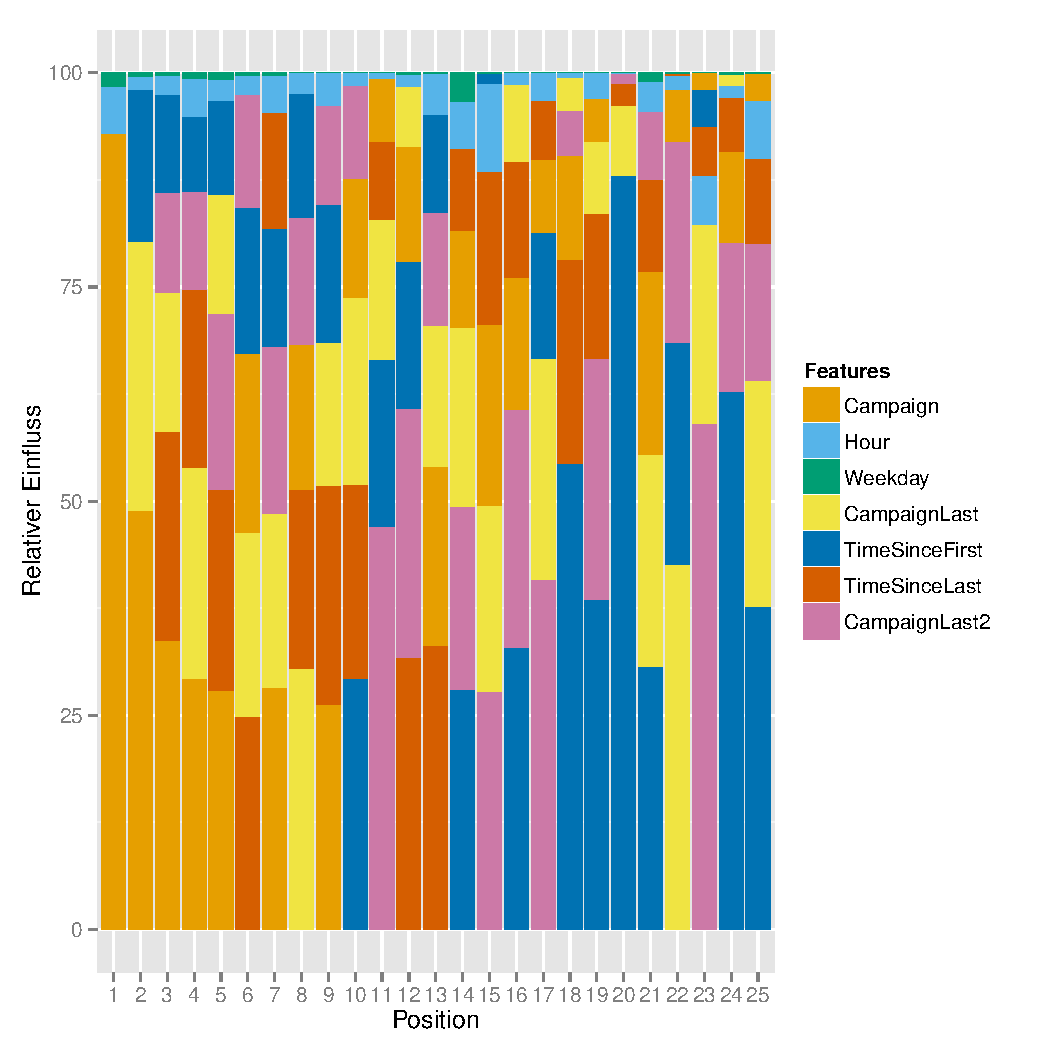
\includegraphics[scale=0.9]{variableImportance.pdf}\caption{Wichtigkeit der Variablen}\label{variable_importance}
\end{figure}
In Abbildung \ref{marg_eff_campaign} sind die marginalen Effekte der Variable \textit{Campaign} für die Positionen eins bis vier, von links oben nach rechts unten, aufgetragen. \textit{Campaign} ist an den ersten vier Positionen das wichtigste Feature. Mit steigender Position verliert die Variable deutlich an Einfluss. Auf der $x$-Achse ist die Art des aktuellen Kontaktpunnktes aufgetragen und auf der $y$-Achse der Marginale Effekt.\\
An Position eins haben die Kampagnen \textit{Affiliate - Rest}, \textit{E-Mailing} und \textit{SEM - Brand} im Vergleich zu den restlichen Kampagnen einen starken, positiven Einfluss auf die Konvertierungswahrscheinlichkeit.
\begin{figure}[H]
	\centering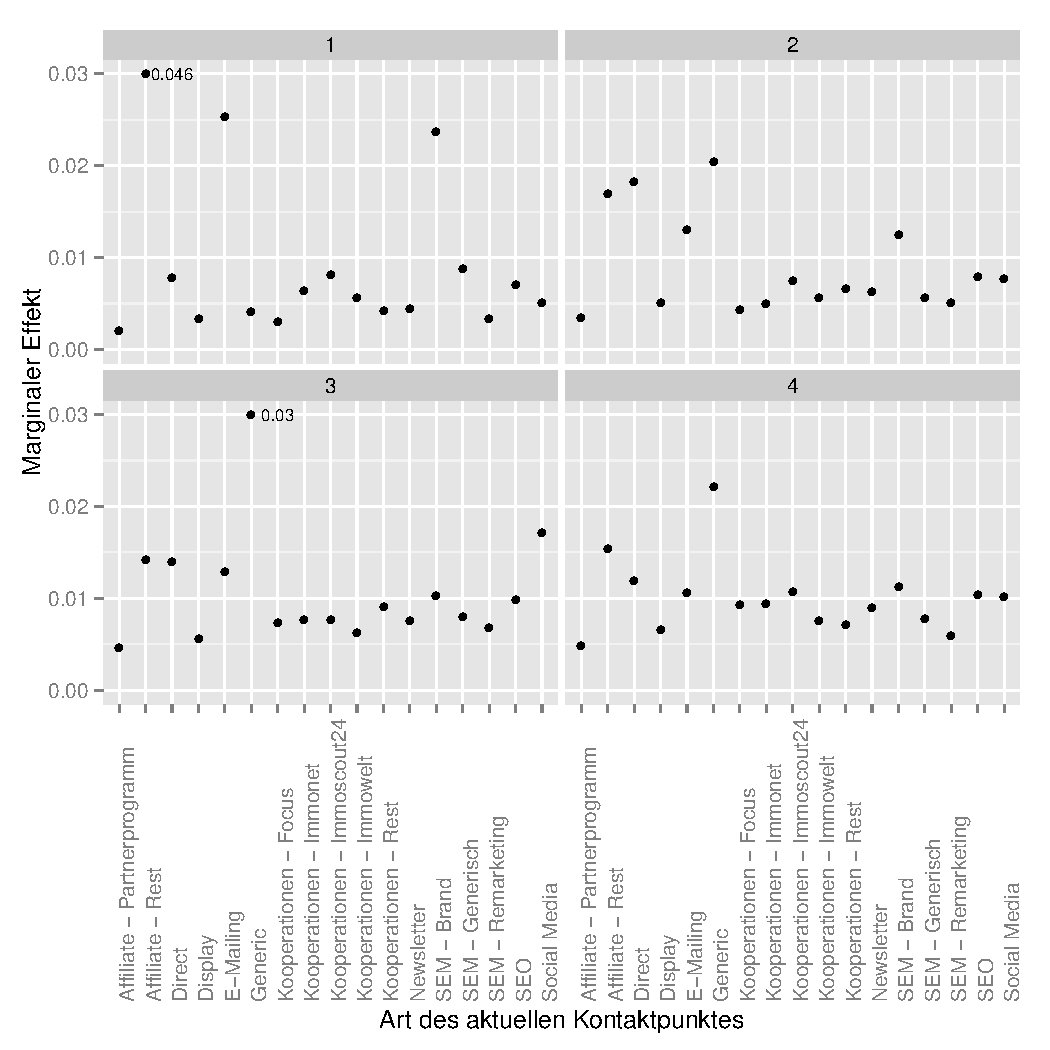
\includegraphics[scale=0.75]{marg_eff_campaign.pdf}\caption[Marginaler Effekt von \textit{Campaign}]{Marginaler Effekt des Features \textit{Campaign} an den Positionen $1$, $2$, $3$ und $4$}\label{marg_eff_campaign}
\end{figure}
\noindent Das heißt das Bereitstellen von Zinsvergleichen, welche das Zinsangebot der Interhyp AG mit deren Wettbewerbern im Vergleich darstellt, durch die Partner unter \textit{Affiliate - Rest} scheint oft an Position $1$ bereits zur Konvertierung zu führen. Die Partner unter \textit{Affiliate - Partnerprogramm}, die hauptsächlich Rechner der Interhyp AG auf ihren Seiten einbinden, teilweise aber auch Banner schalten oder Verlinkungen in Texten unterbringen, haben an Position $1$ einen deutlich geringeren Effekt. \textit{E-Mailing} sind Mails, die an Interessenten, die schon einen Antrag gestellt haben oder ein Infopaket angefordert hatten, versendet werden. Da dieses Klientel sich offentsichtlich bereits intensiv mit einer Baufinanzierung beschäftigt hat, macht es Sinn, dass diese Mails schon nach wenigen Kontakten häufig zu einer Konvertierung führen und dieser Effekt für spätere Positionen schwächer ist. SEM sind bezahlte Suchergebnisse, hauptsächlich auf Google. \textit{SEM - Brand} bedeutet, dass der Suchbegriff das Wort \textit{Interhyp} enthielt. Dieser Effekt ist deutlich größer als für \textit{SEM - Generisch} beziehungsweise \textit{SEM - Remarketing}, wobei ersteres bedeutet, dass etwas wie \textit{Baufinanzierung} gesucht wurde und zweiteres, dass der potentielle Kunde bereits zuvor auf der Seite von Interhyp war und deshalb nochmal eine Einblendung mit Werbung der Interhyp AG bekommen hat.
\begin{figure}[H]
	\centering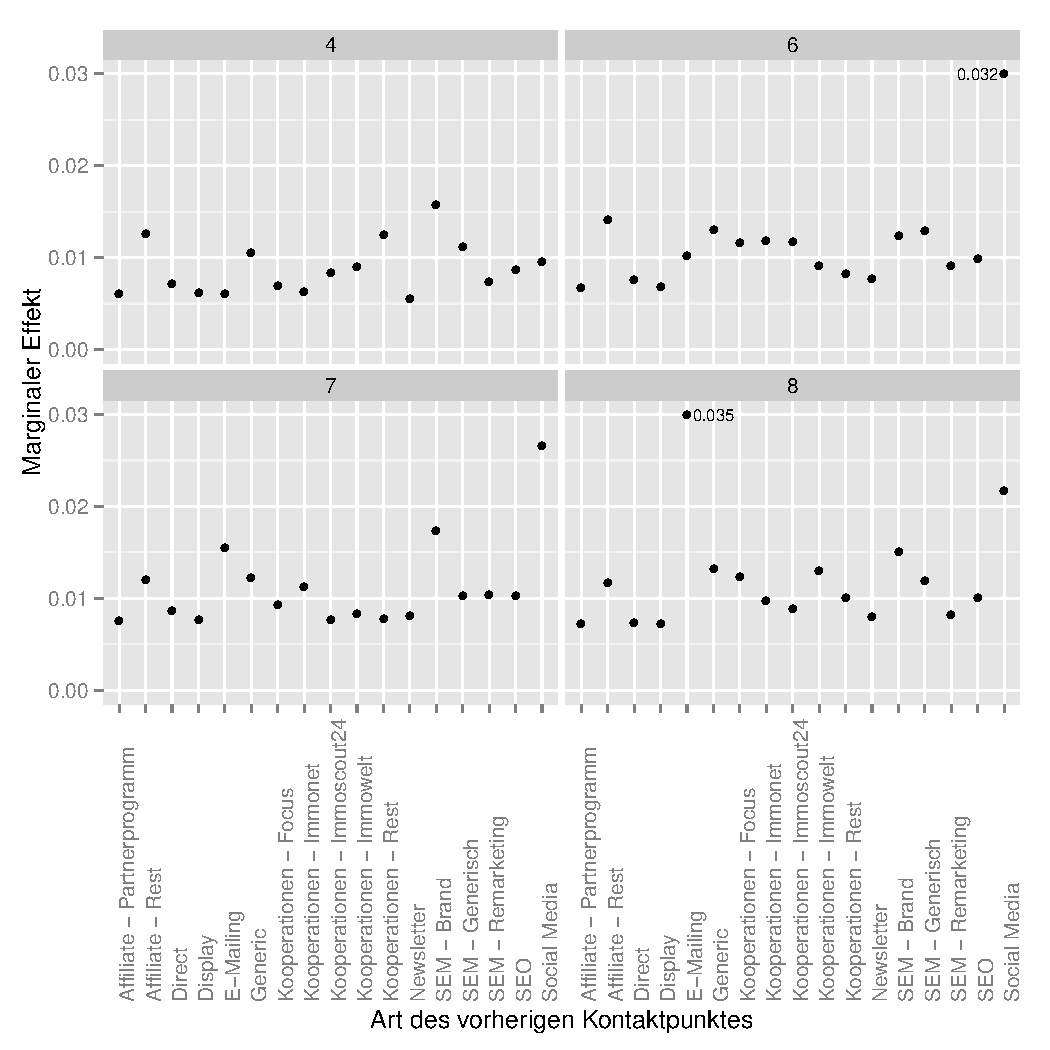
\includegraphics[scale=0.75]{marg_eff_campaignLast.pdf}\caption[Marginaler Effekt von \textit{CampaignLast}]{Marginaler Effekt des Features \textit{CampaignLast} an den Positionen $4$, $6$, $7$ und $8$}\label{marg_eff_campaignLast}
\end{figure}
\noindent An Position $2$ stechen neben \textit{Affiliate - Rest}, \textit{SEM - Brand} und \textit{E-Mailing} auch \textit{Direct} und \textit{Generic} durch ihre Marginalen Effekte leicht hervor. \textit{Direct} bedeutet, dass jemand im Browser direkt \textit{www.interhyp.de} eingegeben hat und \textit{Generic}, dass jemand über einen unbezahlten Link zur Interhyp kam.
Für die Positionen $3$ und $4$ ist vor allem \textit{Generic} wichtig. \textit{Display}, \textit{Social Media}, \textit{SEO} sowie die Kooperationen spielen, neben den bereits erwähnten, keine große Rolle für die ersten vier Positionen.\\
An den Positionen $4$, $6$ und $7$ ist \textit{CampaignLast} das zweitwichtigste Feature sowie an Position $8$ das wichtigste. Dessen marginalen Effekte sind in Abbildung \ref{marg_eff_campaignLast} dargestellt. Hier heben sich teilweise die selben Kategorien hervor, wobei die Unterschiede zwischen den Kampagnen kleiner sind. Überraschend ist, dass hier auch \textit{Social Media} einen starken Effekt hat. Allerdings liegen hierfür kaum Daten vor, wie in Abbildung \ref{campaign} zu erkennen ist.
\begin{figure}[H]
	\centering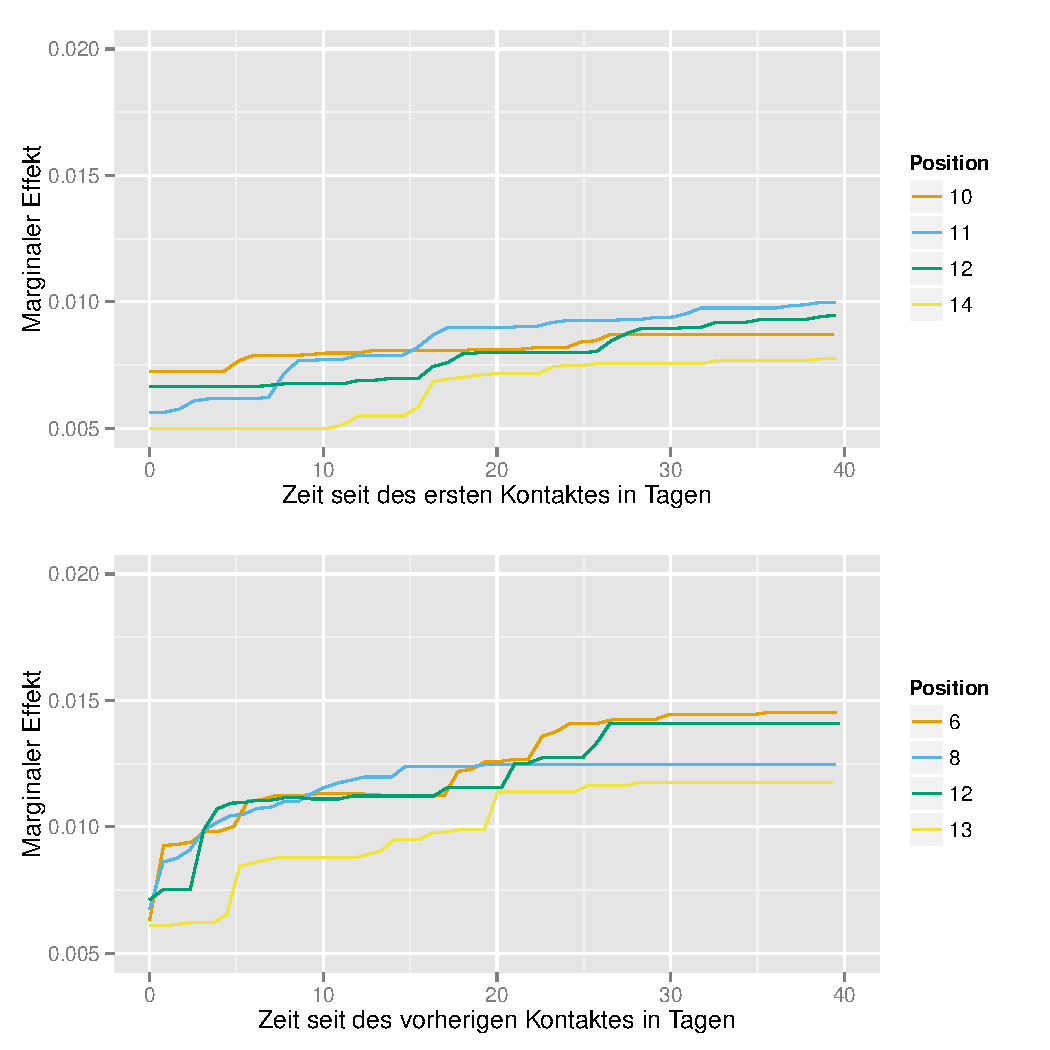
\includegraphics[scale=0.75]{marg_eff_time.pdf}\caption[Marginaler Effekt von \textit{TimeSinceFirst} und \textit{TimeSinceLast}]{Marginaler Effekt des Features \textit{TimeSinceFirst} an den Positionen $10$, $11$, $12$ und $14$ (oben) und des Features \textit{TimeSinceLast} an den Positionen $6$, $8$, $12$ und $13$ (unten)}\label{marg_eff_time}
\end{figure}
\noindent Das Feature \textit{TimeSinceFirst} ist an den Positionen $10$ und $14$ das wichtigste sowie an Position $11$ und $12$ das zweit- beziehungsweise drittwichtigste. \textit{TimeSinceLast} ist an den Positionen $6$, $12$ und $13$ das wichtigste Feature und an Position $8$ das zweitwichtigste Feature. Die marginalen Effekte für diese Positionen sind in Abbilung \ref{marg_eff_time} dargestellt, wobei diese an anderen Positionen ähnlich aussehen. Auf der $x$-Achse ist die Zeit in Tagen aufgetragen und auf der $y$-Achse die Marginalen Effekte. Für beide Features und alle Positionen steigen die marginalen Effekte mit der Zeit, wobei der Effekt bei \textit{TimeSinceLast} etwas größer ist.\\
Dass die Konvertierungswahrscheinlichkeit bei zeitlich längeren Funnels höher ist, könnte man dadurch erklären, dass die Entscheidung für den Bau eines Hauses oder ähnlichem und das damit verbundene Ausfüllen eines Online-Antrages viel Zeit in Anspruch nimmt. Dass für die Zeit seit des vorherigen Kontaktes der selbe Effekt auftritt, könnte man ähnlich erklären. Bei der Entscheidung für eine Baufinanzierung sind viele Dinge zu beachten. So erscheint es plausibel, dass sich interessierte Kunden eine längere Zeit auch offline mit dem Thema beschäftigen und später wieder online den Kontakt zur Interhyp AG suchen.\\
Bis hierhin wurden die Ergebnisse des, auf den Trainingsdaten geschätzten, Modells vorgestellt. Nun soll das Modell auf die Testdaten angewendet werden, um die Prognosegüte zu beurteilen.
\begin{figure}[H]
	\centering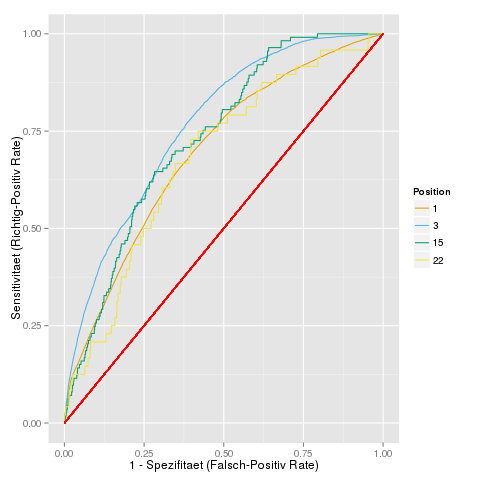
\includegraphics[scale=0.6]{roc.png}\caption[ROC-Kurve]{ROC-Kurve für die Positionen $1$, $3$, $15$ und $22$}\label{roc}
\end{figure}
\noindent Wenn man die geschätzte Prognosefunktion auf die Testdaten anwendet, bekommt man für jede Position und jede ID aus den Testdaten die Hazardrate, das heißt die Wahrscheinlichkeit an einer bestimmten Position zu konvertieren. Diese sind sowohl für konvertierte als auch nicht-konvertierte Funnels sehr niedrig, da die absolute Anzahl an nicht-konvertierten Funnels deutlich überwiegt. Um die Prognosegüte des Modells näher zu betrachten wurde deshalb für jede Position eine ROC-Kurve berechnet. Diese sind in Abbildung \ref{roc} für vier Positionen beispielhaft dargestellt.\\
Auf der $x$-Achse ist der Anteil der nicht-konvertierten Funnels, die als konvertiert vorhergesagt wurden aufgetragen und auf der $y$-Achse der Anteil der konvertierten Funnels, die auch als konvertiert vorhergesagt wurden. Je weiter die ROC-Kurve also oberhalb der roten Diagonalen liegt, desto besser kann das Modell zwischen konvertierten und nicht-konvertierten Funnels trennen. Für Position $3$ liegt die Kurve für alle Punkte überhalb der Kurve von Position $1$. Dies ist dadurch zu erklären, dass an Position $3$ mehr Informationen zur Erstellung des Modells verwendet werden als an Position $1$. Für Position $15$ und $22$ ist das Modell schlechter als an Position $3$. Die Kurven für die späteren Positionen sind deutlich rauher. Dies ist darauf zurück zu führen, dass dort weniger Datenpunkte vorhanden sind. Durch das Einbringen des Offsets kann die Prognoseleistung des Modells allerdings halbwegs konstant gehalten werden.\\
Dies ist in Abbildung \ref{auc} noch deutlicher zu erkennen. Hier ist die Fläche unterhalb der ROC-Kurve (AUC) für jede Position abgebildet. Dieser Wert fällt zwischen Position $15$ und $22$ unter $0.75$ ab, hält sich ansonsten aber relativ konstant auf $0.75$. Das heißt die Wahrscheinlichkeit, dass bei einer konvertierten Beobachtung die Hazardrate größer ist als bei einer nicht-konvertierten Beobachtung ist positionsübergreifend circa $0.75$.
\begin{figure}[H]
	\centering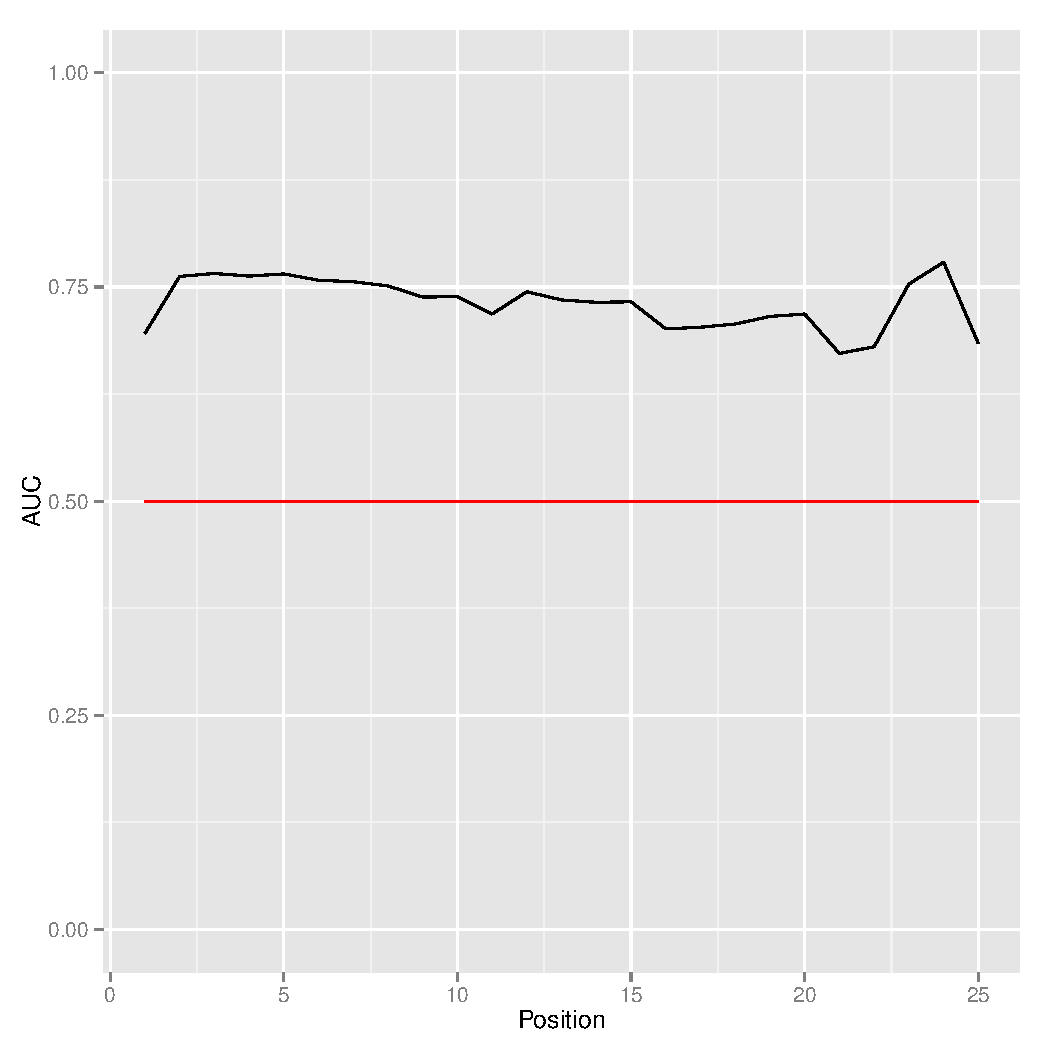
\includegraphics[scale=0.6]{auc.pdf}\caption[AUC-Wert]{AUC für alle Positionen}\label{auc}
\end{figure}

\subsection{Sequential Pattern Mining}\label{ergspm}

Der in Kapitel \ref{spm} beschriebene Algorithmus wurde zunächst seperat auf alle konvertierten sowie nicht-konvertierten Funnels angewendet. Dabei wurden Funnels mit der Länge eins ausgeschlossen, da in diesen offentsichtlich keine interessanten Sequenzen enthalten sein können. Der minimale Support wurde auf $0.05$ gesetzt, so dass nur Sequenzen, die in mindestens $5 \%$ aller Funnels vorkommen, als Ergebnis ausgegeben werden.
\begin{figure}[H]
	\centering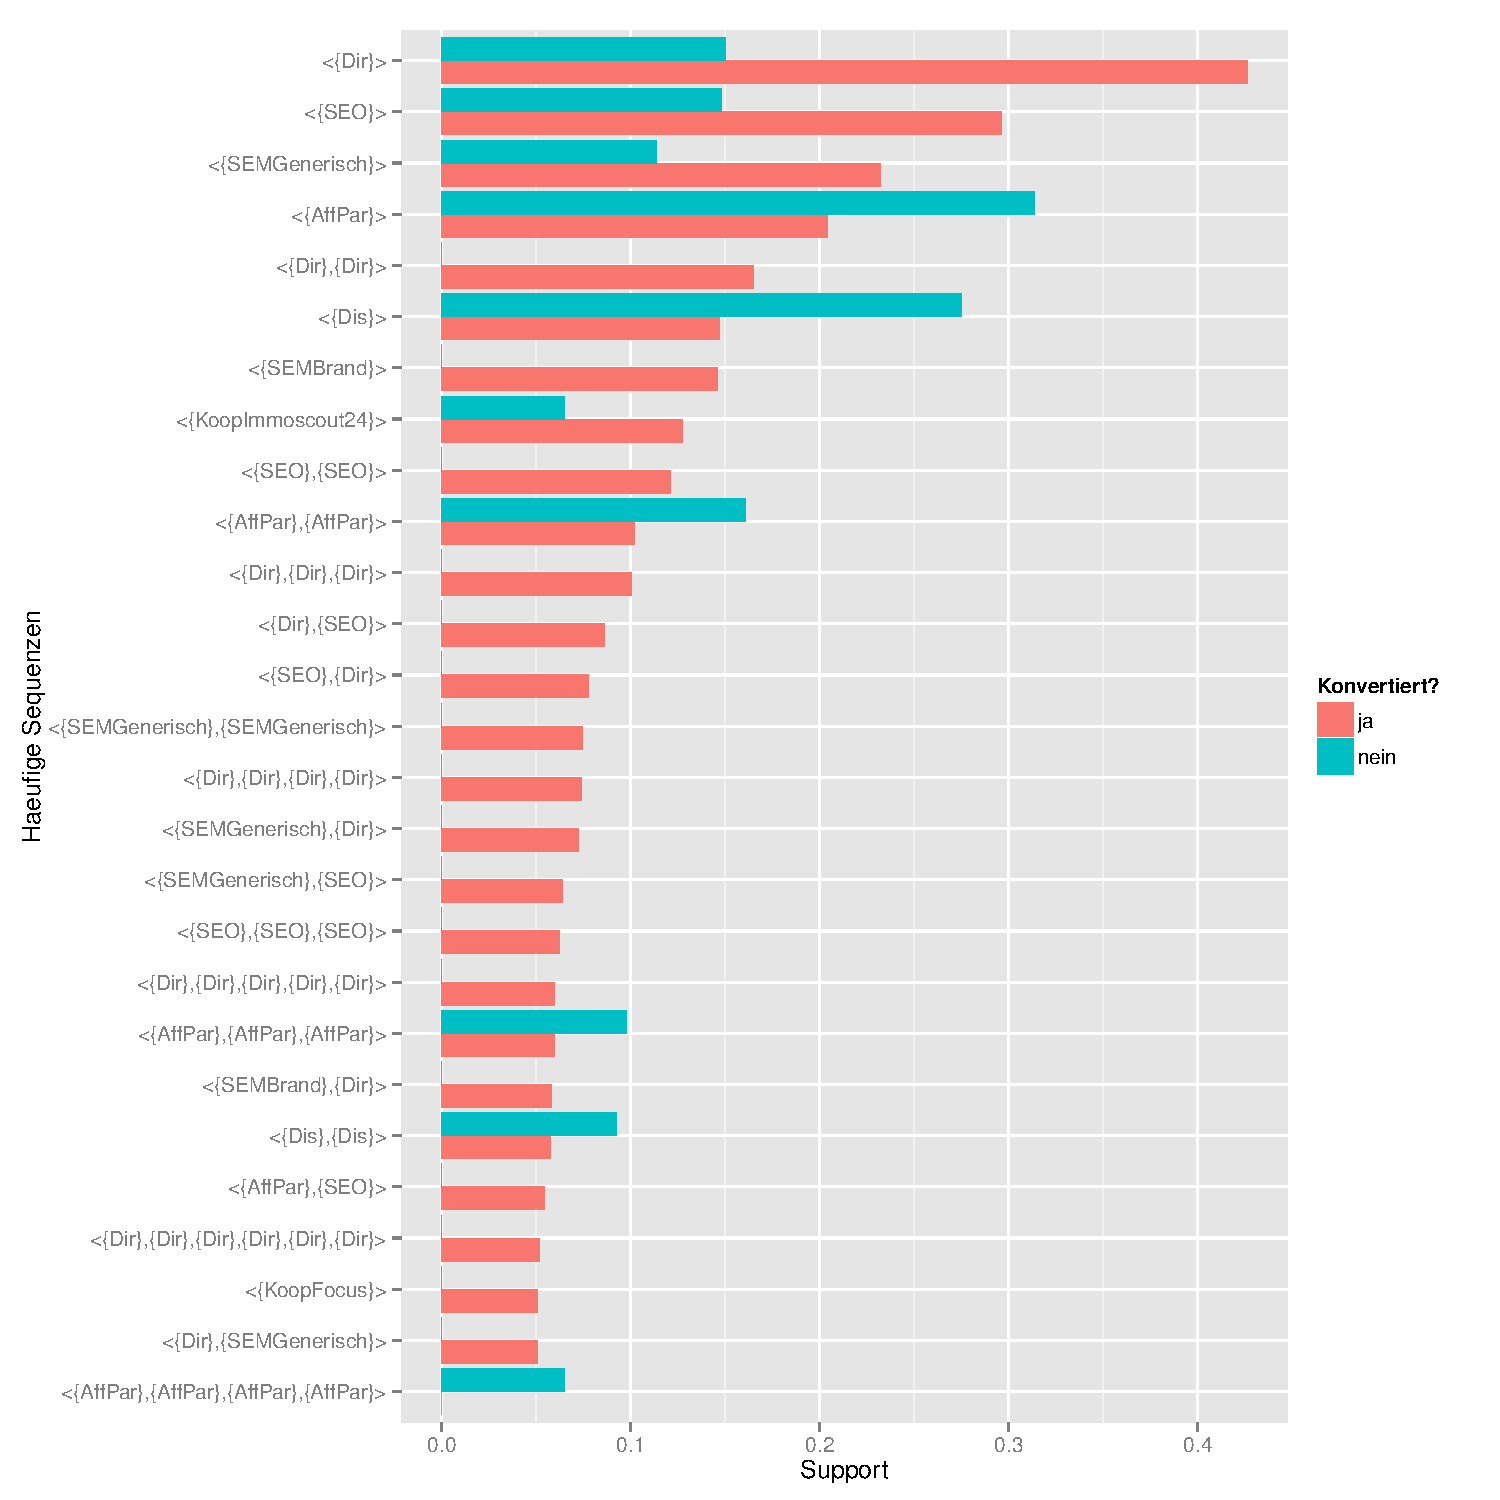
\includegraphics[scale=0.6]{spm_all.pdf}\caption[Häufige Sequenzen]{Häufige Sequenzen in den konvertierten und nicht-konvertierten Funnels}\label{spm_all}
\end{figure}
\noindent In Abbildung \ref{spm_all} sind diese Sequenzen geplottet, wobei auf der $x$-Achse der Suppport aufgetragen ist und die Sequenzen anhand des Supports der Sequenzen in den konvertierten Funnels absteigend geordnet sind. An den Stellen, wo keine Balken geplottet sind, war der Support kleiner als $0.05$. Die Namen der Kampagnen sind teilweise abgekürzt, um die Darstellung zu verbessern. \textit{AffPar} steht für \textit{Affiliate - Partnerprogramm}, \textit{Dir} für \textit{Direct} und \textit{Dis} für \textit{Display}. Außerdem ist zu beachten, dass die Sequenzen nicht exakt in der dargestellten Weise in den Funnels vorkommen müssen, sondern auch Abstände zwischen den aufeinanderfolgenden Kampagnen erlaubt sind.
\begin{figure}[H]
	\centering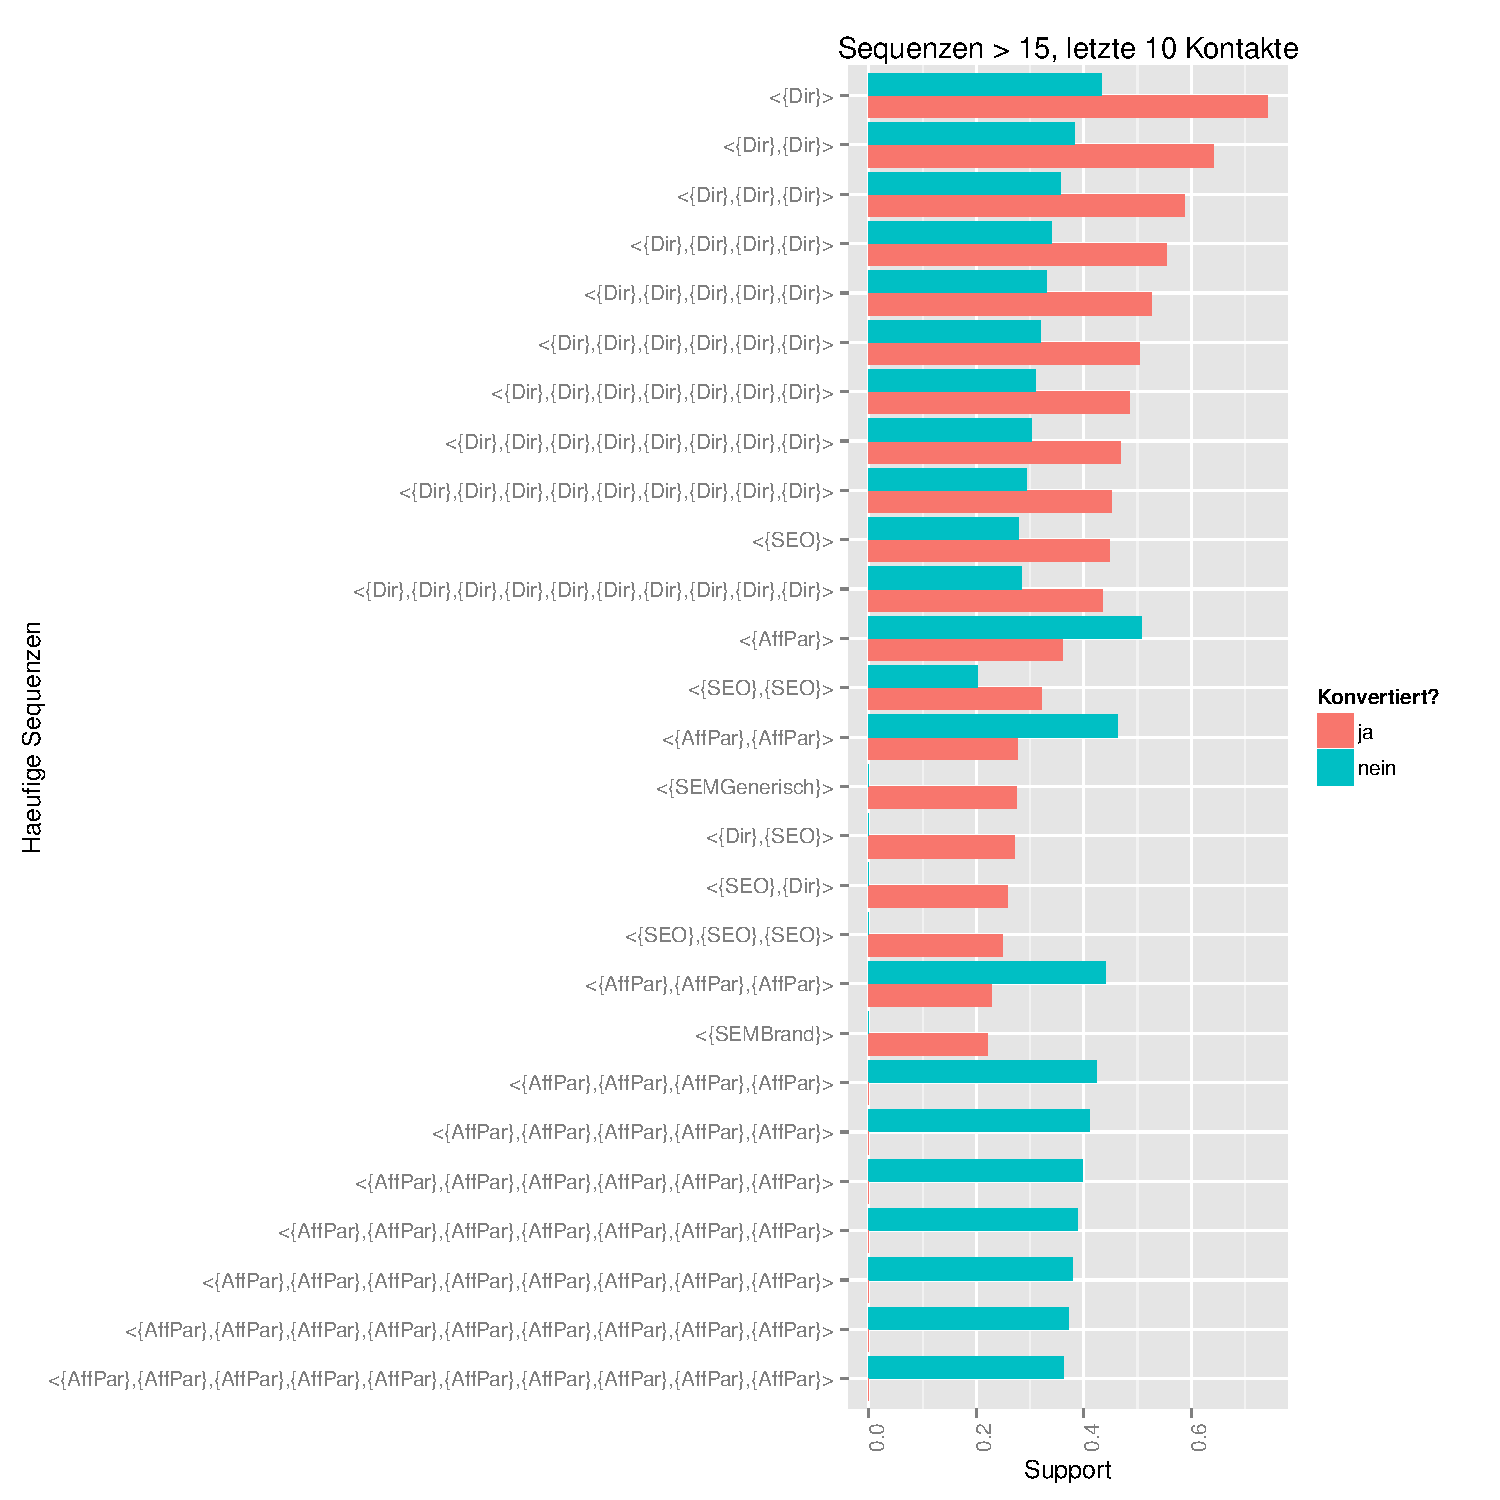
\includegraphics[scale=0.6]{spm_min15.pdf}\caption[Häufige Sequenzen in Funnels mit mindestens $15$ Kontaktpunkten]{Häufige Sequenzen in den konvertierten und nicht-konvertierten Funnels mit mindestens $15$ Kontakten}\label{spm_min15}
\end{figure}
\noindent Der Support von Sequenzen der Länge eins, wie \textit{<\{Dir\}>} oder \textit{<\{SEO\}>}, geben lediglich an, wie groß der Anteil der Funnels ist, die diese Kampagne mindestens einmal enthalten. Interessanter sind Sequenzen, die mindestens zwei Kampagnen enthalten. Hier fällt auf, dass Sequenzen mit wiederholtem \textit{Direct}-Kontakt in den konvertierten Funnels stärker sind. Umgekehrt sind  Sequenzen mit wiederholtem \textit{Affiliate - Partnerprogramm}-Kontakt in den nicht-konvertierten Funnels stärker. Allerdings haben die Sequenzen insgesamt einen sehr geringen Support. Das liegt vor allem daran, dass die Daten zu großem Teil aus sehr kurzen Funnels bestehen (siehe Abbildung \ref{funnelLength}).\\
Deshalb wurde der SPADE-Algorithmus erneut seperat auf konvertierte und nicht-konvertierte Funnel angewendet, wobei dieses mal nur Funnels verwendet wurden, die eine Mindestlänge von $15$ haben. Der minimale Support wurde auf $0.2$ erhöht, um die Anzahl an häufigen Sequenzen zu beschränken. Die Ergebnisse sind in Abbildung \ref{spm_min15} dargestellt.\\
Die Sequenzen haben jetzt teilweise einen Support, der größer als $0.5$ ist, das heißt mehr als die Hälfte der Funnels beinhalten diese Sequenz. Hier ist noch deutlicher zu erkennen, dass die \textit{Direct}-Sequenzen in den konvertierten Funnels stärker sind als in den nicht-konvertierten Funnels. Die \textit{Affiliate - Partnerprogramm}-Sequenzen haben in den nicht-konvertierten Funnels einen Support von ungefähr $40 \%$ und in den konvertierten Funnels einen Support von unter $20 \%$.\\

\subsection{Netzwerk}\label{resultsnetwork}

Mit dem Programm \textit{Gephi} ist es möglich interaktiv mit dem Netzwerk zu arbeiten. Eine komplette Analyse des Netzwerkes würde den Rahmen dieses Berichtes sprengen. Deshalb soll hier nur beispielhaft, anhand einiger Grafiken, dargestellt werden, welche Ergebnisse man aus dem Netzwerk ziehen kann. Dafür wurde ein Ausschnitt an Position $2$ gewählt. Eine genauere Anleitung zur Verwendung von \textit{Gephi} ist zudem in Kapitel \ref{anhang} zu finden.

\subsubsection*{Relative Ausgänge}

Zunächst werden die relativen Ausgänge präsentiert, das heißt die Gewichte aller Kanten, die einen Knoten verlassen, ergeben in der Summe $1$.\\
Abbildung \ref{out_labels} enthält den Ausschnitt des Netzwerkes an Position $2$ mit den relativen Ausgängen. Die Knoten sind farblich codiert und mit Labels versehen. Am rechten Bildrand ist noch eine Kampagne der ersten Position \textit{SEO\_1} zu erkennen. Von dort und den anderen Kampagnen der ersten Position führen die Kanten zu den Kampagnen der zweiten Position in der Mitte der Abbildung. Für Funnels, die mehr als zwei Kontaktpunkte haben gehen die Kanten von diesen Kampagnen zu den Knoten der dritten Positionen jenseits des linken Bildrandes. Die Kampagne \textit{Affiliate - Partnerprogramm\_3} ist noch zu erkennen.\\
Funnels, die lediglich über zwei Kontaktpunkte verfügen, enden in \textit{Fail\_2} im Falle einer Nicht-Konvertierung beziehungsweise in \textit{Success\_2} im Falle einer Konvertierung.
\begin{figure}[H]
	\centering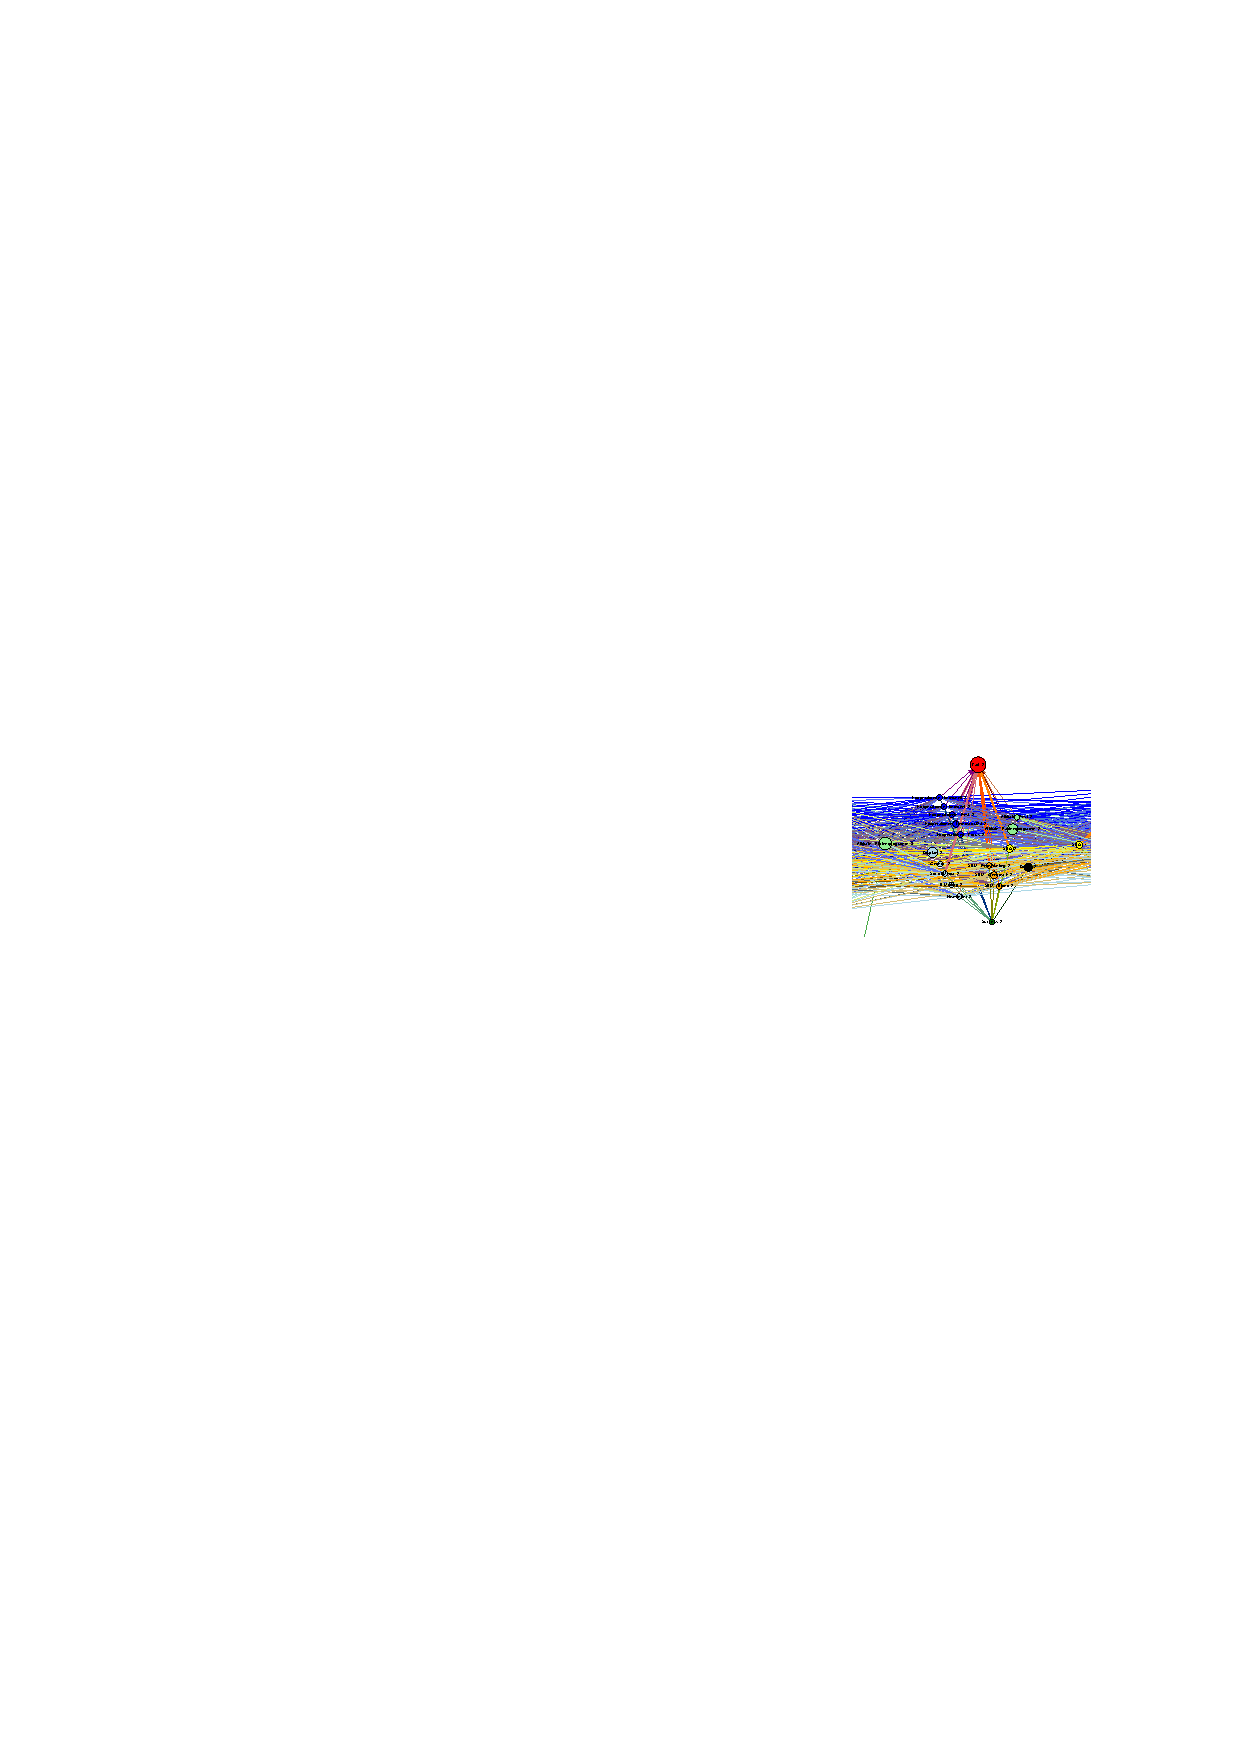
\includegraphics[scale=2.3]{out_labels.pdf}\caption[Relative Ausgänge]{Auschnitt des Netzwerkes an Position $2$ mit relativen Ausgängen}\label{out_labels}
\end{figure}
Die Dicke der Kanten hängt von deren Gewichtung ab. Abbildung \ref{out_filter_2_succ} enthält den selben Ausschnitt, wobei nun ein Filter von $0.02$ auf die Kanten angewendet wurde. Somit sind nur noch Kanten abgebildet, deren Gewicht größer als $0.02$ ist. Durch das Auswählen des Knoten \textit{Success\_2} werden alle Knoten hervorgehoben, die nach der Anwendung des Filters noch durch eine Kante mit \textit{Success\_2} verbunden sind.
\begin{figure}[H]
	\centering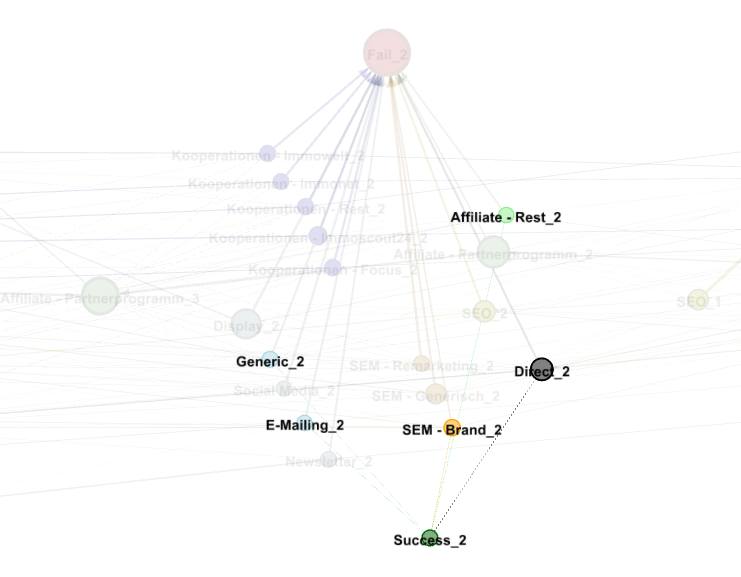
\includegraphics[scale=0.35]{out_filter_2_succ.png}\caption[Relative Ausgänge mit Filter $0.02$]{Auschnitt des Netzwerkes an Position $2$ mit relativen Ausgängen, Filter $0.02$ und Fokus auf den konvertierten Funnels}\label{out_filter_2_succ}
\end{figure}
Das heißt über $2 \%$ aller Nutzer, die als zweiten Kontaktpunkt $Direct$ haben, konvertieren an der zweiten Position. Selbiges gilt für \textit{Affiliate - Rest}, \textit{Generic}, \textit{SEM - Brand} und \textit{E-Mailing}. Durch Veränderung der Filter und weiterer Einstellungen können die Ergebnisse auch noch genauer betrachtet werden. Wie bereits erwähnt, ist in Kapitel \ref{anhang} ein Tutorial dazu vorhanden.\\
Interessant ist an dieser Stelle, dass die fünf hervorgehobenen Kampagnen gleichzeitig die fünf stärksten Kampagnen bei den Marginalen Effekten des Features \textit{Campaign} an Position $2$ sind. Das heißt die Ergebnisse des Survival-Modells können durch die Betrachtung des Netzwerkes überprüft und bestätigt werden.\\
Abbildung \ref{out_filter_50_fail} enthält erneut den selben Ausschnitt des Netzwerkes, wobei nun ein Filter von $0.5$ angewendet wurde und der Fokus auf den nicht-konvertierten Funnels liegt. Von den hervorgehobenen Knoten enden also jeweils mindestens die Hälfte der Beobachtungen ohne Konvertierung.\\
Analog zu der Betrachtung von \textit{Success\_2} oder \textit{Fail\_2} können auch die Kampagnen durch Auswählen näher betrachtet werden. Durch die positionsübergreifende Betrachtung können zudem die häufigen Sequenzen, die mittels des Sequential-Pattern-Mining Algorithmus ermittelt wurden, erkannt werden.
\begin{figure}[H]
	\centering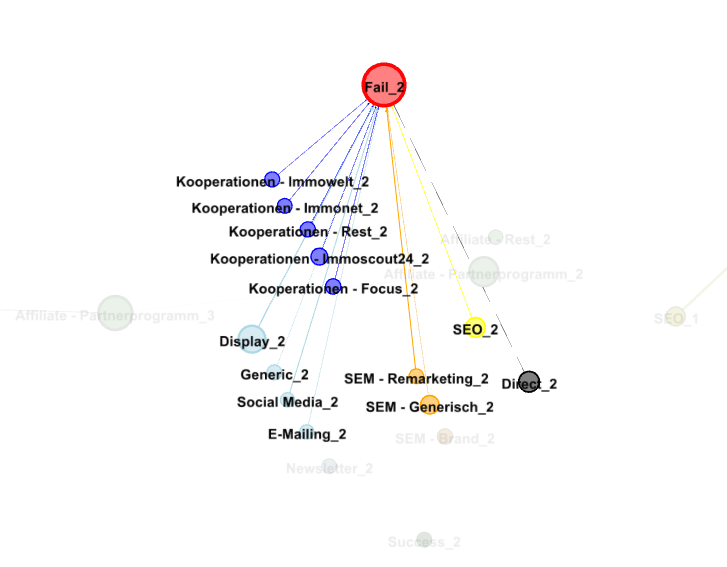
\includegraphics[scale=0.35]{out_filter_50_fail.png}\caption[Relative Ausgänge mit Filter $0.5$]{Auschnitt des Netzwerkes an Position $2$ mit relativen Ausgängen, Filter $0.5$ und Fokus auf den nicht-konvertierten Funnels}\label{out_filter_50_fail}
\end{figure}

\subsubsection*{Relative Eingänge}

In diesem Abschnitt wird erneut Position $2$ betrachtet, wobei die Kanten nun anhand der relativen Eingänge gewichtet sind. Das heißt die Gewichte aller Kanten, die in einen bestimmten Knoten gehen, ergeben aufsummiert $1$. Abbildung \ref{in_labels} enthält den Ausschnitt des Netzwerkes. Am rechten beziehungsweise linken Bildrand ist erneut eine Kampagne von Position $1$ beziehungsweise $3$ zu erkennen. Die Farben und Beschriftungen der Knoten sind die selben wie in Abbildung \ref{out_labels}. 
\begin{figure}[H]
	\centering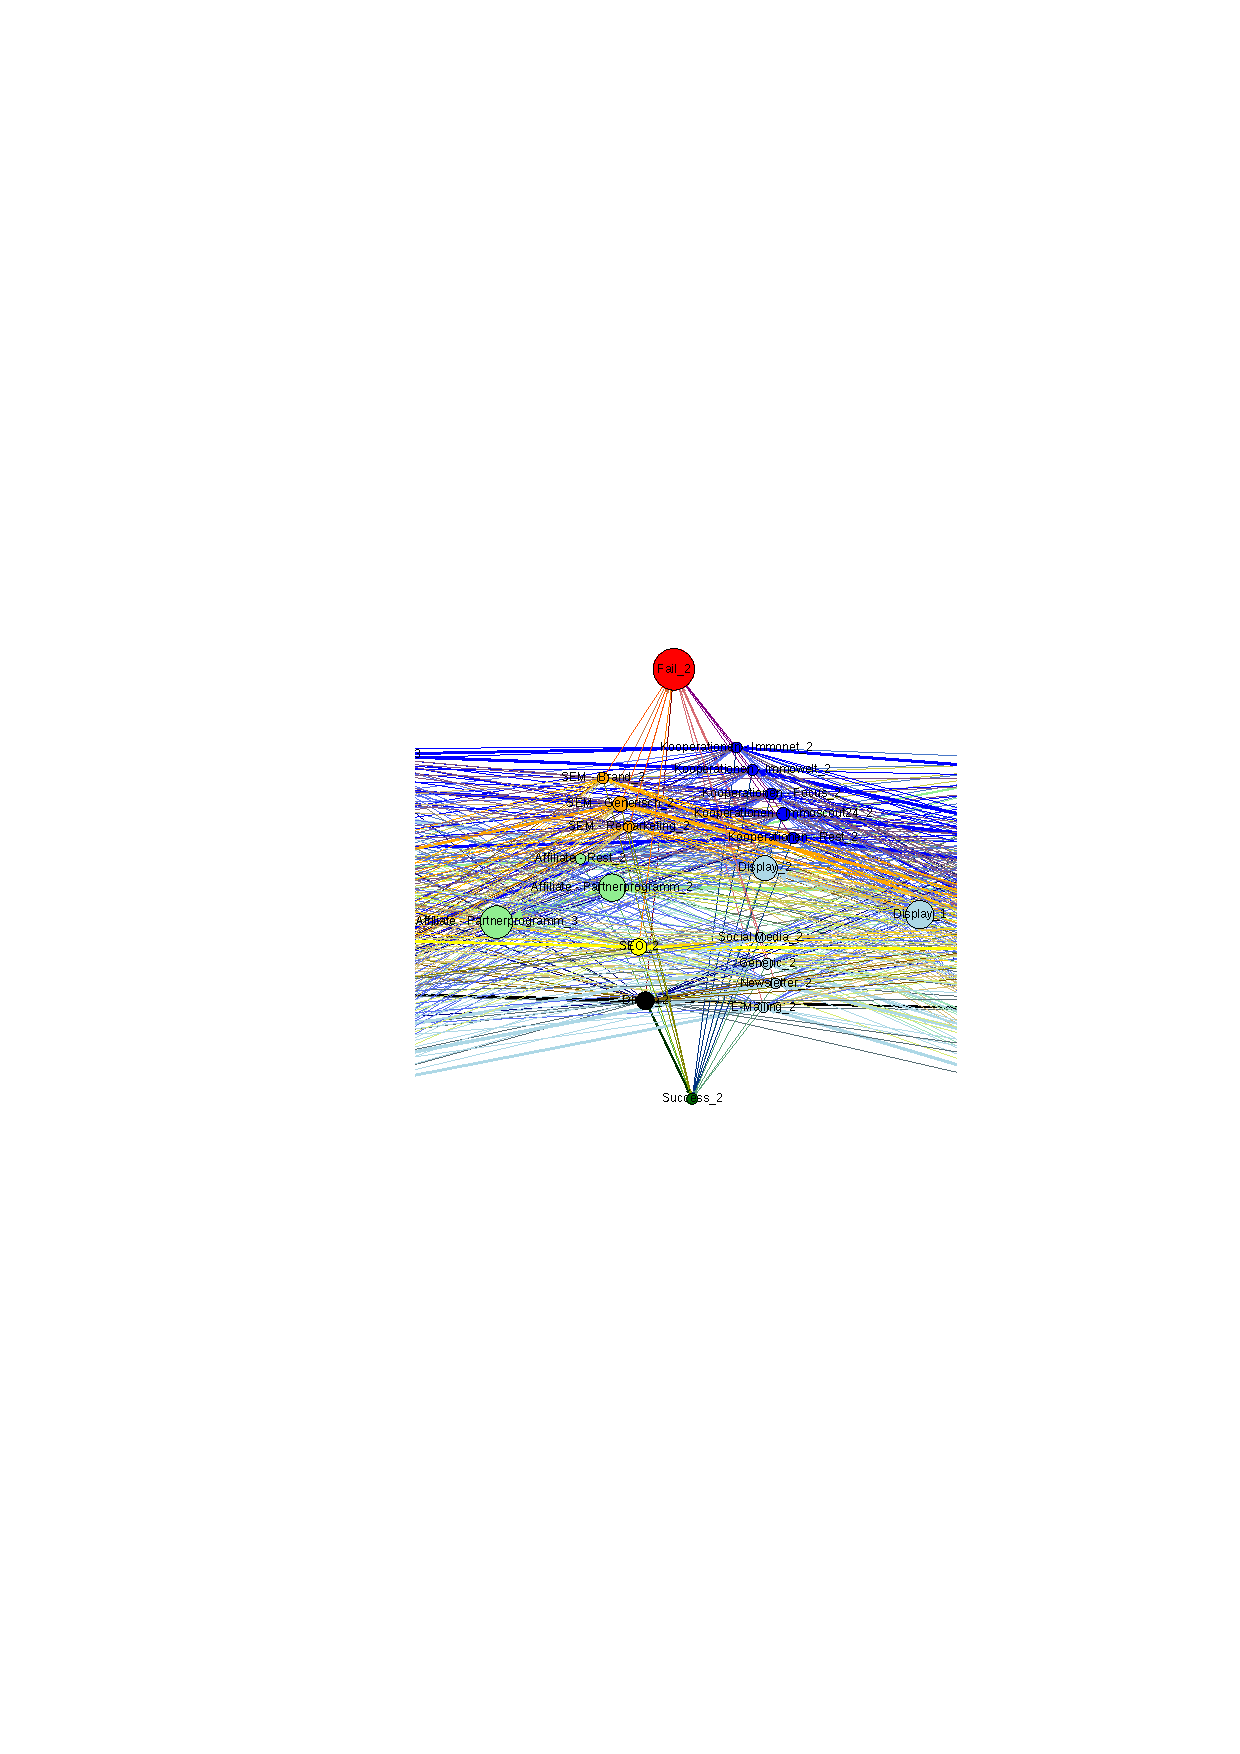
\includegraphics[scale=0.9]{in_labels.pdf}\caption[Relative Eingänge]{Auschnitt des Netzwerkes an Position $2$ mit relativen Eingängen}\label{in_labels}
\end{figure}
\noindent Auf diesen Ausschnitt wurde ein Filter von $0.1$ angewendet, wobei der Fokus auf den konvertierten Funnels liegt. Der resultierende Graphh ist in Abbildung \ref{in_filter_10_succ} zu sehen.
\begin{figure}[H]
	\centering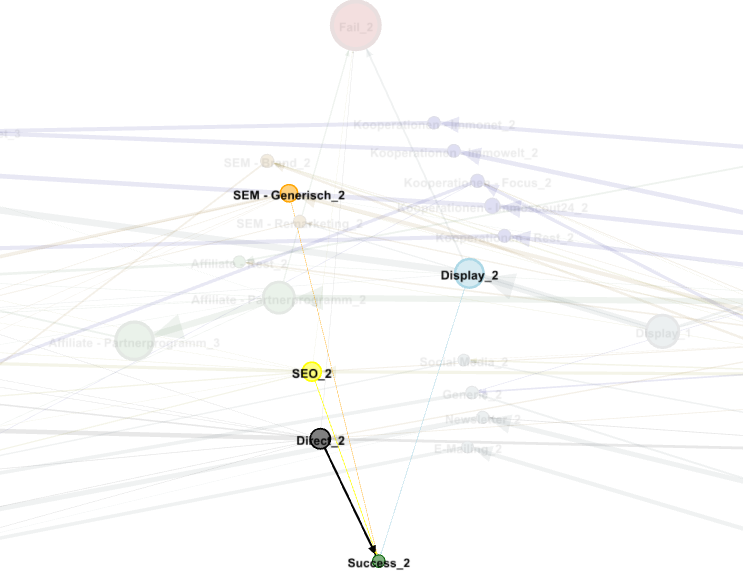
\includegraphics[scale=0.35]{in_filter_10_succ.png}\caption[Relative Eingänge mit Filter $0.1$ und Fokus auf Konvertierten]{Auschnitt des Netzwerkes an Position $2$ mit relativen Eingängen, Filter $0.1$ und Fokus auf den konvertierten Funnels}\label{in_filter_10_succ}
\end{figure}
\noindent Die hervorgehobenen Knoten \textit{SEM-Generisch\_2}, \textit{Display\_2}, \textit{SEO\_2} und \textit{Direct\_2} machen jeweils mehr als $10 \%$ der konvertierten Funnels aus, die aus zwei Kontaktpunkten bestehen. Das heißt hier kann nun betrachtet werden, aus welchen Kampagnen des letzten Kontaktpunktes sich die Menge der konvertierten beziehungsweise nicht-konvertierten Funnels zusammensetzen. Zudem ist es auch möglich eine Kampagne zu markieren, so dass erkennbar wird, aus welchen Kampagnen der vorherigen Position, sich diese zusammensetzt. Im Gegensatz dazu, war die Interpretation im vorherigen Kapitel eine andere. Dort wurde betrachtet, wohin die Nutzer von einem Knoten aus gehen.\\
Abbildung \ref{in_filter_10_fail} enthält den selben Ausschnitt mit dem selben Filter von $0.1$, wobei nun die nicht-konvertierten Funnels betrachtet werden. Das heißt von den Funnels, die nach zwei Kontaktpunkten ohne Konvertierung abbrechen, haben jeweils mindestens $10\%$ als letzten Kontaktpunkt \textit{Affiliate - Partnerprogramm\_2}, \textit{Display\_2}, \textit{SEO\_2} oder \textit{Direct\_2}.
\begin{figure}[H]
	\centering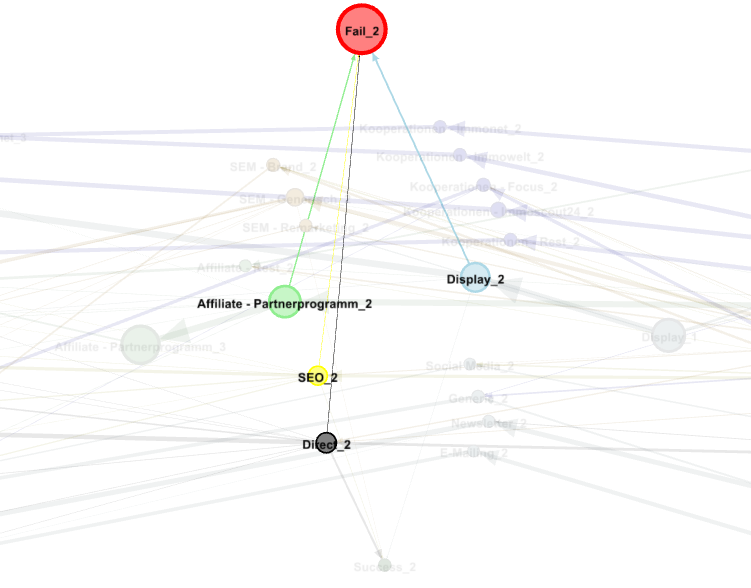
\includegraphics[scale=0.35]{in_filter_10_fail.png}\caption[Relative Eingänge mit Filter $0.1$ und Fokus auf Nicht-Konvertierten]{Auschnitt des Netzwerkes an Position $2$ mit relativen Eingängen, Filter $0.1$ und Fokus auf den nicht-konvertierten Funnels}\label{in_filter_10_fail}
\end{figure}
\section{Zusammenfassung}\label{zusammenfassung}

An dieser Stelle sollen die angewendeten Methoden und Ergebnisse noch einmal kurz zusammengefasst werden.\\
Es wurde ein zeitdiskretes Survival-Modell aufgestellt, dass für jede Beobachtung an jeder Position die Konvertierungswahrscheinlichkeit schätzt. Dieses Modell kann als Klassifikator in konvertierte und nicht-konvertierte Funnels fungieren. Die Prognosegüte konnte vor allem durch die Anwendung von Stochastic Gradient Boosting und die Einführung des Offsets verbessert werden. Außerdem liefern die Marginalen Effekte der Features eine gute Interpretationsmöglichkeit der Prädiktorfunktion.\\
Die wichtigsten Ergebnisse an dieser Stelle sind, dass die Kampagnen \textit{Affiliate - Rest}, \textit{E-Mailing}, \textit{SEM - Brand}, \textit{Direct} und \textit{Generic} im Vergleich zu den restlichen Kampagnen besonders gut für die Konvertierung funktionieren. Außerdem haben Funnels mit einer längeren Beobachtungsspanne und einer niedrigeren Frequenz von Kontaktpunkten eine höhere Konvertierungswahrscheinlichkeit.\\
Die Einführung von Interaktionen in das Modell hat zu einer Verschlechterung der Prognoseleistung geführt und wurde deshalb nicht weiter verfolgt. Außerdem konnten die \textit{Views} aufgrund der Datenlage in den statistischen Analysen nicht berücksichtigt werden.\\
Mit dem Sequential Pattern Mining-Algorithmus sollten häufige Sequenzen in den Funnels entdeckt werden. Von den resultierenden Ergebnissen sind die \textit{Direct}-Sequenzen in den konvertierten und die \textit{Affiliate - Partnerprogramm}-Sequenzen in den nicht konvertierten Funnels erwähnenswert. Allerdings ist zu berücksichtigen, dass zwischen den einzelnen Elementen der Sequenzen auch andere Kampagnen erlaubt sind. Ein weiterer Ansatz wäre nur diejenigen Funnels zu berücksichtigen, die die Sequenzen in der exakten Reihenfolge ohne Lücken vorweisen. Bei der gegebenen Datenlage würde das allerdings zu einer drastischen Reduzierung des Supports der Sequenzen führen, zumal der Support der häufigen Sequenzen aufgrund der überwiegenden Anzahl an kurzen Funnels ohnehin nicht sehr groß ist. Um interessantere Ergebnisse zu erlangen, wurden die Daten deshalb noch in Form eines Netzwerkes visualisiert.\\
Dieses Netzwerk erlaubt die Visualisierung der gesamten Daten. Außerdem können durch die Gewichtung der Kanten mit den relativen Ein- und Ausgängen wertvolle Informationen aus den Daten gezogen werden. Mit Hilfe des, in diesem Bericht bereitgestellten, Tutorials (siehe Kapitel \ref{anhang}) ist ein interaktives Arbeiten mit dem Netzwerk sowie eine weiterführende Erforschung der Daten möglich.
\section{Elektronischer Anhang}\label{anhang}

\subsection{Verzeichnisstruktur}
Abbildung \ref{verz} zeigt die Verzeichnisstruktur des elektronischen Anhangs. Dieser soll hier noch erklärt werden.
\begin{figure}[H]
\dirtree{% dieses Kommentar-Zeichen ist noetig, da der erste Charakter in der Umgebung ein '.' sein muss
.1 consulting/.
.2 raw\_data/.
.2 r\_data/.
.2 sql\_scripts/.
.2 r\_scripts/.
.3 support\_functions/.
.2 r\_results/.
.3 descriptive/.
.3 gbm\_no\_offset/.
.3 gbm\_no\_offset\_interactions/.
.3 gbm\_offset/.
.3 gbm\_offset\_bag/.
.3 gbm\_offset\_interactions/.
.3 spm/.
.2 network/.
.3 gephi/.
.3 network\_data/.
.2 presentation.pdf.
.2 report.pdf.
.2 README.pdf.
}
\caption{Verzeichnisstruktur des Projekts}\label{verz}
\end{figure}
Die rohen Daten, die von der Refined Labs GmbH bereitgestellt wurden, sind im Ordner \textit{raw\_data} enthalten und im Ordner \textit{r\_data} sind die vorverarbeiteten Daten im \textit{RData}-Format abgespeichert. Der Ordner \textit{sql\_scripts} enthält die SQL Skripte, die für die Vorverarbeitung der Daten verwendet wurden. Die R Skripte zur weiteren Vorverarbeitung der Daten, zur deskriptiven Analyse, zur Schätzung des zeitdiskreten Survival-Modells mittels Stochastic Gradient Boosting, zum Sequential Pattern Mining sowie zur Erstellung des Netzwerkes sind im Ordner \textit{r\_scripts} gespeichert. Der Unterordner \textit{support\_functions} enthält zudem einige Hilfsfunktionen.\\
Die Ergebnisse sind in dem Ornder \textit{r\_results} gespeichert. Der Unterordner \textit{descriptive} enthält die in Kapitel \ref{descriptiv} vorgestellten Grafiken als \textit{pdf}-Dateien, wobei die Namen der Dateien aus den Namen der Features resultieren.\\
Der Ordner \textit{spm} enthält die Ergebnisse des Sequential Pattern Mining-Algorithmus im \textit{RData}-Format sowie als Plot, wie in Kapitel \ref{ergspm} vorgestellt. Die Dateien \textit{spadeFail\_all.RData} und \textit{spadeSucc\_all.RData} sind die Ergebnisse des SPADE-Algorithmus in den nicht-konvertierten und konvertierten Funnels, wobei die kompletten Daten berücksichtigt wurden, und \textit{spm\_all.pdf} ist die Visualisierung der Ergebnisse in Form eines Barplots. Außerdem wurde der Algorithmus nur auf Funnels mit mindestens $10$ beziehungsweise $15$ Kontaktpunkten angewendet. Die Namen dieser Ergebnis-Dateien sind analog mit den Endungen \textit{min10} beziehungsweise \textit{min15}.\\
Der Ordner \textit{gbm\_offset} enthält die Ergebnisse des Survival-Modells, die in diesem Bericht vorgestellt wurden. Die Dateien \textit{dataTrain.RData} und \textit{dataTest.RData} enthalten die Trainings- und Testdaten. Die Datei \textit{model.RData} enthält das eigentliche Ergebnis des Modells und \textit{predTrain.RData} und \textit{predTest.RData} enthalten die Vorhersagen auf den Daten anhand des Modells. Die Vorhersagen auf den Trainingsdaten wurden lediglich für den Offset verwendet und die Vorhersagen auf den Testdaten wurden zur Bewertung der Prognosegüte des Modells verwendet. Außerdem enthält der Ordner einige Plots zur Visualisierung der Ergebnisse. Unter anderem sind hier die marginalen Effekte aller Features für jede Position enthalten.\\
Zusätzlich zu den Ergebnissen, die in diesem Bericht vorgestellt wurden, sind noch Ergebnisse des Survival-Modells mit anderen Parametereinstellungen im Ordner \textit{r\_results} bereitgestellt. Diese Parametereinstellungen haben allerdings stets zu schlechteren Resultaten geführt als die Ergebnisse in dem Ordner \textit{gbm\_offset}. Der Ordner \textit{gbm\_no\_offset} enthält Ergebnisse des Modells ohne Offset und \textit{gbm\_no\_offset\_interactions} Ergebnisse ohne Offset und mit Interaktionen, das heißt einer \textit{interaction.depth} von $2$. Für den Ordner \textit{gbm\_offset\_bag} wurde lediglich die \textit{bag.fraction} auf $1$ gesetzt und die Ergebnisse sind nahezu identisch zu \textit{gbm\_offset}. Ergebnisse mit Offset und Interaktionen sind im Ordner \textit{gbm\_offset\_interactions} zu finden.\\
Für die Ergebnisse des Netzwerkes wurde ein seperater Ordner \textit{network} angelegt. Der Unterordner \textit{gephi} enthält die Installationsdateien für das Open Source-Programm \textit{Gephi}, dass für das Arbeiten mit dem Netzwerk benötigt wird. Die \textit{dmg}-Datei ist für Computer mit dem Betriebssystem \textit{Mac OSX}, die \textit{gz}-Datei ist für Linux und die \textit{exe}-Datei für Windows. Alternativ können die Installationsdateien auch auf \textit{https://gephi.github.io/} heruntergeladen werden.\\
Nach der Installation von \textit{Gephi} kann das Netzwerk in das Programm gelesen werden. Der Ordner \textit{network\_data} enthält dafür sechs Dateien. Das gesamte Netzwerk mit allen Positionen kann mit den Dateien \textit{relative\_ausgänge.gexf} oder \textit{relative\_eingänge.gexf} geladen werden. Die Dateien \textit{relative\_ausgänge\_pos\_10.gexf} und \textit{relative\_eingänge\_pos\_10.gexf} enthalten das selbe Netzwerk, allerdings nur für die ersten $10$ Positionen. Im nächsten Kapitel wird beschrieben, wie man mit diesen Dateien in \textit{Gephi} arbeiten kann. Die Dateien mit der Endung \textit{Layout} enthalten zudem ein Layout des Netzwerkes der ersten $10$ Positionen, das bereits eine übersichtliche Betrachtung des Netzwerkes ermöglicht. Für dieses Layout wurde die Anordnung der Knoten nach dem Anwenden des \textit{ForceAtlas2}-Algorithmus noch manuell bearbeitet.\\
Neben den bereits beschriebenen Ordnern sind im Hauptverzeichnis noch die Folien des Vortrages vom 12.08.2014 im Institut für Statistik, dieser Bericht sowie dieser elektronische Anhang als \textit{README}-Datei gespeichert.

\subsection{Tutorial zu Gephi}

\newpage
\listoftables
\listoffigures
\newpage
\printbibliography

\end{document}
